% Template LaTeX document for CSSR4Africa Deliverables
% Adapted from documents prepared by EPFL for the RobotCub project
% and subsequently by the University of Skövde for the DREAM project
%
% DV 28/06/2023

\documentclass{CSSRforAfrica}

\usepackage{array}
\usepackage{caption}
\usepackage{dirtree}
\usepackage{float}
\usepackage{fontenc}
%\usepackage{geometry}
\usepackage{graphicx}
\usepackage{latexsym}
\usepackage{listings}
%\usepackage{lmodern}
\usepackage{longtable}
\usepackage{pdflscape}
\usepackage{pdfpages}
\usepackage[table,dvipsnames,svgnames]{xcolor}
\usepackage{tikz}
\usepackage[titletoc,title]{appendix}
\usepackage{url}
\usepackage{tabularx,colortbl}
\usepackage{verbatim}
\usepackage{subcaption}
\usepackage{multicol}
\usepackage[hidelinks,colorlinks=false]{hyperref}
\usetikzlibrary{shapes.geometric, positioning, arrows.meta,shapes,arrows, calc}
\captionsetup[figure]{format=hang}
\definecolor{backcolour}{rgb}{0.95,0.95,0.95} 
\definecolor{codegreen}{rgb}{0,0.6,0}
\definecolor{codepurple}{rgb}{0.5,0.0,0.5}
\definecolor{greenyellow}{rgb}{0.8, 0.7, 0.10}

\lstdefinestyle{withoutNumbering}{
    backgroundcolor=\color{backcolour},   
    commentstyle=\color{codegreen},
    keywordstyle=\color{magenta},
    stringstyle=\color{codepurple},
    %%basicstyle=\ttfamily\small,
    basicstyle=\ttfamily\scriptsize,
    breakatwhitespace=false,         
    breaklines=true,                 
    captionpos=b,                    
    keepspaces=true,                 
    showspaces=false,                
    showstringspaces=false,
    showtabs=false,                  
    tabsize=2
}

% Define custom colors
\definecolor{backcolour}{rgb}{0.95,0.95,0.92}
\definecolor{codegreen}{rgb}{0,0.6,0}
\definecolor{codeblue}{rgb}{0,0,0.8}
\definecolor{codepurple}{rgb}{0.58,0,0.82}
\definecolor{darkred}{rgb}{0.6,0,0.0}
\definecolor{brown}{rgb}{0.6,0.4,0.2}

% Define a custom XML language with keywords for different node types
\lstdefinelanguage{XMLCustom}{
    morestring=[b]",
    morestring=[b]',
    morecomment=[s]{<!--}{-->},
    sensitive=true,
    % Control Flow Nodes:
    morekeywords={
      Sequence, Fallback, Parallel, Inverter, RetryUntilSuccessful, KeepRunningUntilFailure
    },
    % Tree Nodes:
    alsoletter={<},
    morekeywords=[2]{
      root, BehaviorTree, SubTree, START_OF_TREE
    },
}

% Define the style for XML code
\lstdefinestyle{XMLStyle}{
    language=XMLCustom,
    backgroundcolor=\color{backcolour},
    basicstyle=\ttfamily\small,
    commentstyle=\color{codegreen},
    keywordstyle=\color{codeblue}\bfseries,
    keywordstyle=[2]\color{brown}\bfseries,
    stringstyle=\color{codepurple},
    breaklines=true,
    breakatwhitespace=true,
    showstringspaces=false,
    captionpos=b,
    escapeinside={(*@}{@*)},
    literate={<}{{\textcolor{darkred}{<}}}1 {>}{{\textcolor{darkred}{>}}}1 {</}{{\textcolor{darkred}{</}}}2
}



\hypersetup{
    colorlinks=true,
    linkcolor=black,
    filecolor=magenta,      
    urlcolor=blue,
    citecolor=blue,
    pdfpagemode=FullScreen
    }



\newcommand{\blank}{~\\}
\newcommand{\checkbox}{{~~~~~~~\leavevmode \put(-7,-1.5){  \huge $\Box$  }}}


 
%% Directory Tree Font
%\renewcommand*\DTstyle{\rmfamily\footnotesize}
%\renewcommand*\DTstyle{\sffamily\footnotesize}
%\renewcommand{\DTstyle}{\small\ttfamily}
\renewcommand{\DTstyle}{\footnotesize \ttfamily}
%\renewcommand{\DTstyle}{\scriptsize \ttfamily}

\captionsetup[figure]{format=hang}


%\usepackage{titlesec}
%\setcounter{secnumdepth}{4}
%\titleformat{\paragraph}
%{\normalfont\normalsize\bfseries}{\theparagraph}{1em}{}
%\titlespacing*{\paragraph}{0pt}{10pt}{5pt}


\begin{document}
\input{epsf}

%%
%% SHOULD NOT NEED TO BE CHANGED BEFORE THIS POINT
%% ------------------------------------------------
%%

\deliverable{D5.4.2}              
\title{D5.4.2 Robot Mission Language}   

\leadpartner{Carnegie Mellon University Africa (for Wits)}      
\partner{Carnegie Mellon University Africa}                               

\revision{1.7}                           
\deliverabledate{30/06/2024}  
\submissiondate{05/03/2025}  
\revisiondate{04/05/2025}      
\disseminationlevel{PU}
\responsible{Tsegazeab Tefferi, CMU-Africa}


%%
%% Create the titlepage
%%

\maketitle
 

\section*{Executive Summary}
%===============================================================
\label{executive_summary}
%%\addcontentsline{toc}{section}{Executive Summary}
 
This deliverable  represents the outcome of Task 5.4.2.  It comprises three elements: (i) a mode of abstract modelling ---  behavior trees --- that can be used to formally specify the interactions in the use case scenarios  and enact them in a culturally sensitive manner using the  culture knowledge base and an environment knowledge base, 
%%(ii)  a specification of the two use case scenarios using behavior trees, 
(ii) an environment knowledge base file with the  information required to complete the robot mission, and 
(iii) the documented software required to compile a C++ helper class  {\small \tt EnvironmentKnowledgeBase} to read the environment knowledge base file, store the knowledge, and make the knowledge accessible through a suite of access methods. As such, this deliverable, along with Deliverable D6.1 Use Case Implementation with the specification of the two use case scenarios using behavior trees, provides the input for the development in Task 5.4.3 of an interpreter that can translate this abstract specification into robot actions, thereby  enacting the use case scenarios defined in Tasks 2.1, 2.2, and 2.3 and documented in  Deliverables D2.1, D2.2, and D2.3.  




\begin{comment}
The knowledge base itself, i.e., a C++ object instantiation of the {\small \tt EnvironmentKnowledgeBase} class, is determined by the contents of a configuration file that  contains two key-value pairs.  
One key-value pair  specifies the filename of the file in which the knowledge is stored.  
One key-value pair specifies whether diagnostic data is to be printed to the terminal (e.g., {\small \tt verboseMode true}).
The configuration file is named {\small \tt environmentKnowledgeBaseConfiguration.ini}.  
\end{comment}


In the CSSR4Africa work plan, this deliverable  and Deliverables D5.4.1 and D5.4.3 were  assigned to the University of the Witswatersrand. However, the material in this  report was developed and written by Carnegie Mellon University Africa. This was necessary because, due to extensive delays in the delivery of the Pepper robot to the University of the Witswatersrand, little or no progress had been made. Since the cultural knowledge ontology and culture knowledge base, the robot mission language, and the robot mission interpreter are essential for integrating and demonstrating the use case scenarios,  Carnegie Mellon University Africa took joint responsibility for these three deliverables (among others, specificially D5.5.2.1, D5.5.4,  D6.1, and D6.2). Since this involved a significant amout of additional, unplanned effort, only one use case, the laboratory tour,  has been implemented to date, leaving the second use case, the receptionist, to be implemented later.


\pagebreak
\tableofcontents
\newpage


\section{Introduction}
%===============================================================
 \label{section:introduction}


This deliverable documents the outcome of Task 5.4.2 which is concerned with providing a methodology, or language, for specifying robot missions. Section \ref{section:specification} provides the foundational knowledge necessary for understanding the specification and implementation of robot missions using behavior trees. Behavior trees have emerged as a robust and flexible alternative to state machines, offering a structured and intuitive approach for formally specifying interactions and decision-making processes within use-case scenarios \cite{Ghzoulietal2023}. This section begins with 
%%a detailed introduction to 
a short overview behavior trees (Section \ref{section:overview}). Subsequently, the execution flow of behavior trees is discussed (Section \ref{section:flow}), clarifying how nodes are evaluated and executed. The structural components essential to behavior trees are then systematically detailed (Section \ref{section:structure}). Finally, the Groot2 tool, a graphical interface specifically developed to facilitate the design and management of behavior trees, is introduced (Section \ref{section:groot}) along with a practical demonstration of its usage provided by designing a simple behavior tree example. 

The actual specification of the robot missions for the two use case scenarios defined in Tasks 2.1, 2.2, and 2.3 and documented in  Deliverables D2.1, D2.2, and D2.3 is detailed in Deliverable D6.1 Use Case Implementation.

Since we are particularlarly focused on enacting these missions in a culturally sensitive manner, we require both a cultural knowledge ontology \&  culture knowledge base,  and an environment knowledge ontology \& environment knowledge  base.
The former is described in Deliverable D.5.4.1, while the latter is described in Section \ref{section:knowledge_base} of this deliverable. 

The deliverable concludes with Section \ref{section:implementation} which addresses the implementation of the environment knowledge base and, specifically, with the description of a C++ helper class  to read the environment knowledge base file, store the knowledge, and make the knowledge accessible through a suite of access methods.  As such, it  provides the input for the development in Task 5.4.3 of an interpreter that can translate the  abstract behavior tree specifications shown in ``Implementation'' into robot actions, thereby  enacting the use case scenarios defined in Tasks 2.1, 2.2, and 2.3 and documented in  Deliverables D2.1, D2.2, and D2.3.  

In the work plan, this deliverable and deliverable D5.4.3 were assigned to the University of the Witswatersrand. However, the material in this report was developed and written by Carnegie Mellon University Africa. This was necessary because of unavoidable delays in the completion of the associated task by Wits, and because the robot mission language and the robot mission interpreter, are essential for integrating and demonstrating the use case scenarios. 

%%\newpage

\section {Specification of Robot Missions with Behavior Trees} %% Find a better title for it
%=====================================
\label{section:specification}

\subsection{Behavior Trees}
\label{section:overview}
A behavior tree is a powerful and flexible framework for designing the control architecture of an autonomous agent, such as a robot or a virtual character in a computer game. Behavior trees decompose complex tasks into a hierarchy of simpler, modular actions and decisions. This hierarchical structure typically consists of \textbf{composite nodes}, which control the flow between tasks and \textbf{mission/leaf nodes}, which execute the actual actions or check conditions \cite{Ghzoulietal2023,DortmansPunter2022}.

\subsection{Flow of Execution}
\label{section:flow}
The execution of a behavior tree begins at its root node, which periodically generates signals called ``\textbf{Ticks}'' at a defined frequency. These ticks propagate downward through the tree, following the traversal logic defined by control-flow nodes. When ticked, each node executes its associated task; leaf nodes specifically perform robotic actions or evaluate conditions, returning one of three possible statuses: \textbf{Running}, if the task is still ongoing, \textbf{Success}, if the goal has been achieved, or \textbf{Failure}, if the task cannot be completed. Unlike state machines, Behavior Trees do not allow direct jumps or ``goto'' statements; instead, composite nodes locally influence the traversal logic, guiding the flow of execution dynamically and modularly \cite{Ghzoulietal2020,Iovinoetal2020}.

The variant of behavior trees used in robotics is predominantly a time-triggered, activity-based behavioral modeling language. Rather than explicitly shifting control tokens or managing states as in traditional control loops, this approach periodically triggers the entire model at fixed intervals, similar to clock-driven circuits. Each tick initiates a full traversal of the behavior tree, dynamically branching according to various node types \cite{Ghzoulietal2023}. In contrast, behavior tree implementations in video games use event driven programming as opposed to time-triggered controls
 \cite{Ghzoulietal2020,UnrealEngineBehaviorTree}.

\subsection{Structure}
%=============
\label{section:structure}

\subsubsection{Composite Nodes}
%----------------------------
Composite nodes are internal nodes in a behavior tree that manage the control flow among their child nodes. They do not execute actions or evaluate conditions directly. Instead, they define the order and conditions under which their children are ticked (activated), ensuring that the overall decision-making process follows a structured pattern.

\newpage



\paragraph{Root}~\\
The Root node serves as the entry point for every traversal of the behavior tree. It has exactly one child node and is re-entered at each epoch. The tree is traversed from the Root to the leaf nodes and back, following a depth-first approach.
It is typically represented as an inverted triangle shape with the label ``Root'' at the center; see Fig.~\ref{fig:root}.


\begin{figure}[h]
    \centering
    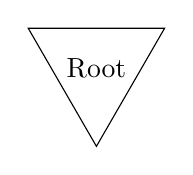
\begin{tikzpicture}
        \node (rootshape) [draw,
                           shape=regular polygon,
                           regular polygon sides=3,
                           rotate=180,
                           minimum size=2cm] {};
        \node at (rootshape.center) {Root};
    \end{tikzpicture}
    \caption{Root node of a behavior tree.}
    \label{fig:root}
\end{figure}




\paragraph{Sequence} ~\\
The Sequence node is a composite node that enforces a strict order of execution among its children. When ticked, it processes its child nodes sequentially from left to right. The Sequence node behaves as follows.
\begin{itemize}
    \item It sends a tick to the first child.
    \item If the child returns \textbf{Success}, the tick is passed to the next child.
    \item If a child returns either \textbf{Failure} or \textbf{Running}, the Sequence node immediately returns that status and halts further processing.
    \item Only if every child returns \textbf{Success} does the Sequence node return \textit{Success}.
\end{itemize}
This design makes the Sequence node ideal for modeling tasks that require multiple steps to be completed in a specific order. While many representations depict the Sequence node with a (\texttt{``Seq''}) label inside a box, alternative symbols --- such as a rectangle containing a right-pointing arrow (\texttt{``→''}) to indicate directional flow --- may also be used, depending on the chosen visual convention; see Fig.~\ref{fig:sequence}.


%\begin{figure}[htbp]
\begin{figure}[th]
\vspace{5mm}
    \centering
    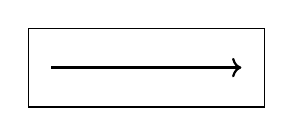
\begin{tikzpicture}
        \node[draw, rectangle, minimum width=3cm, minimum height=1cm] (rect) {};
        \draw[->, thick] ($(rect.west)+(0.3,0)$) -- ($(rect.east)+(-0.3,0)$);
    \end{tikzpicture}
    \caption{Sequence node of a behavior tree.}
    \label{fig:sequence}
\end{figure}




\paragraph{Fallback}~\\
The Fallback node, also known as the Selector, is a composite node that provides an alternative execution path among its children. When ticked, it processes its children sequentially from left to right with the following behavior.\\
\begin{itemize}
    \item It sends a tick to the first child.
    \item If the child returns \textbf{Failure}, it proceeds to tick the next child.
    \item If a child returns either \textbf{Success} or \textbf{Running}, the Fallback node immediately returns that status and stops processing further children.
    \item The Fallback node returns \textbf{Failure} only if all its children return \textbf{Failure}.
\end{itemize}
This design makes the Fallback node ideal for situations where multiple alternative behaviors are available, and success is achieved as soon as one alternative succeeds. It is commonly represented by a box containing the label ``?''; see Fig.~\ref{fig:fallback}.

%\begin{figure}[htbp]
\begin{figure}[h]
\vspace{5mm}
    \centering
    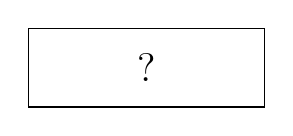
\begin{tikzpicture}
        %%\node[draw, rectangle, minimum width=4cm, minimum height=2cm, align=center,font=\Large] {?};
        \node[draw, rectangle, minimum width=3cm, minimum height=1cm, align=center,font=\Large] {?};
    \end{tikzpicture}
    
    \caption{Fallback node of a behavior tree.}
    \label{fig:fallback}
\end{figure}



\paragraph{Parallel}~\\
The Parallel node is a composite node that simultaneously triggers all of its child nodes and aggregates their outcomes to determine its own status. Its behavior is as follows.
\begin{itemize}
    \item The node sends a tick to every child at the same time.
    \item A user-defined threshold \(M\) is set (with \(M \leq N\), where \(N\) is the total number of children). 
    \item The Parallel node returns \textbf{Success} if at least \(M\) children return \textbf{Success}.
    \item It returns \textbf{Failure} if at least \(N - M + 1\) children return \textbf{Failure}.
    \item If neither condition is met, the node returns \textbf{Running}.
\end{itemize}
It is important to note that ``parallel" does not always mean that the children are executed concurrently; some implementations may process the children sequentially while simulating parallel behavior \cite{Ghzoulietal2020,FacontiGithubComment}.
The Parallel node is typically symbolized by a rectangle that contains the two right directed arrows in parallel inside of it; see Fig.~\ref{fig:parallel}.


%\begin{figure}[htbp]
\begin{figure}[th]
\vspace{5mm}
    \centering
    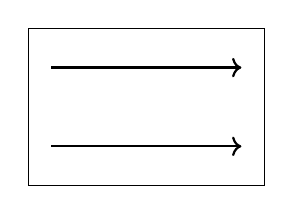
\begin{tikzpicture}
        \node[draw, rectangle, minimum width=3cm, minimum height=2cm] (rect) {};
        \draw[->, thick] ($(rect.west)+(0.3,0.5)$) -- ($(rect.east)+(-0.3,0.5)$);
        \draw[->, thick] ($(rect.west)+(0.3,-0.5)$) -- ($(rect.east)+(-0.3,-0.5)$);
    \end{tikzpicture}
    \caption{Parallel node of a behavior tree.}
   \label{fig:parallel}
\end{figure}



\paragraph{Decorator}~\\
Decorator nodes are unary composite nodes that modify the control flow or data of their single child. They wrap around another node and adjust its return status according to user-defined rules. The are many types of decorator nodes but the common examples include:
\begin{itemize}
    \item \textbf{Inverter:} Flips the return status of its child, returning \textbf{Success} if the child fails and \textbf{Failure} if the child succeeds.
    \item \textbf{Succeeder:} Always returns \textbf{Success}, regardless of the child's actual return status.
    \item \textbf{Repeat:} Acts like a for-loop by repeatedly triggering its child for a predetermined number of ticks. It increments an internal counter on each tick, succeeds (and resets the counter) when a set bound is reached, or fails (and resets the counter) if the child fails.
\end{itemize}
Decorator nodes are typically represented as a rhombus (or diamond) containing the symbol for the specific type of decorator; see Fig.~\ref{fig:decorator}.


%\begin{figure}[htbp]
\begin{figure}[h]
\vspace{5mm}
    \centering
    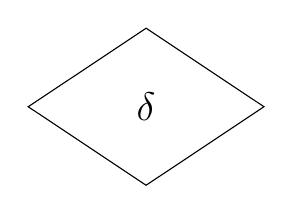
\begin{tikzpicture}
        \node[draw, diamond, aspect=2, minimum width=3cm, minimum height=2cm, align=center, font=\Large] {$\delta$};
    \end{tikzpicture}
    
    \caption{Condition node of a behavior tree. Label indicates the type of decorator.}
    \label{fig:decorator}
\end{figure}

%\newpage

\subsubsection{Leaf Nodes} 
%----------------------
\label{section:leaf_nodes}
Leaf nodes represent the terminal elements of a behavior tree and serve as the interface between the tree's decision-making process and the environment. They are responsible for executing specific operations that directly affect the system or agent. Importantly, unlike composite or control flow nodes, the logic behind leaf nodes is not predefined; it is left for the user to implement. This means that it's upto the programmers to tailor the exact actions or conditions to their specific application needs.

 

\paragraph{Action Nodes}~\\
An Action node executes a command when it receives a tick signal. This command is defined by the user and can be any arbitrary operation that affects the system. For instance, an action node might be programmed to initiate navigation to a certain location, make a certain gesture or process sensor data. The node actively monitors the progress of the command, as follows.
\newpage

\begin{itemize}
    \item \textbf{Execution:} Upon receiving a tick, the node triggers the user-defined command.
    \item \textbf{Status Returns:}
    \begin{itemize}
        \item \textbf{Success:} Returned when the command completes successfully.
        \item \textbf{Failure:} Returned if the command encounters errors or the desired outcome is not achieved.
        \item \textbf{Running:} Returned while the command is still being executed, indicating that the operation is ongoing.
    \end{itemize}
    \item \textbf{Representation:} Typically depicted as a box containing the label of the action; see Fig. \ref{fig:action}.
\end{itemize}


    %\begin{figure}[htbp]
    \begin{figure}[h]
        \centering
        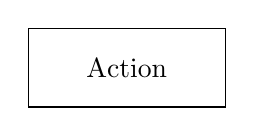
\begin{tikzpicture}
            \node[draw, rectangle, minimum width=2.5cm, minimum height=1cm, align=center] {Action};
        \end{tikzpicture}
        \caption{Action node of a behavior tree. Label describes action performed.}
        \label{fig:action}
    \end{figure}


\paragraph{Condition Nodes}~\\
A Condition node evaluates a proposition when it receives a tick signal. The specific logic for this evaluation is defined by the user, allowing the condition to be customized according to the application’s requirements. For example, a condition node might check if a person is present, or verify whether a variable meets a certain threshold.
\begin{itemize}
    \item \textbf{Evaluation:} The node performs a user-defined check to determine whether the condition holds true.
    \item \textbf{Status Returns:}
    \begin{itemize}
        \item \textbf{Success:} Returned if the condition is met.
        \item \textbf{Failure:} Returned if the condition is not met.
    \end{itemize}
    \item \textbf{No Running Status:} Unlike Action nodes, Condition nodes complete their check immediately and do not return a \textbf{Running} status.
    \item \textbf{Representation:} Typically depicted as a diamond containing the label of the condition; see Fig. \ref{fig:condition}.     
\end{itemize}

    \begin{figure}[h]
        \centering
        
\begin{tikzpicture}
            \node[draw, diamond, aspect=2, minimum width=2.5cm, minimum height=1cm, align=center] {Condition};
        \end{tikzpicture}
        \caption{Condition node of a behavior tree. Label describes the condition to be checked.}
        \label{fig:condition}
    \end{figure}


%\newpage
\subsection{Groot2}
%============
\label{section:groot}

To implement the robot mission interpreter within the CSSR4Africa software ecosystem, which serves as the ROS node responsible for reading and executing behavior trees, we selected \textbf{BehaviorTree.CPP 4.6} as our library. The rationale behind this choice is detailed in \textbf{D5.4.3 Robot Mission Interpreter}. BehaviorTree.CPP is an open-source C++ library that facilitates the implementation, reading, and execution of behavior trees. These trees are defined using a domain-specific scripting language based on XML \cite{Ghzoulietal2023}. Although XML files can be edited with any text editor, BehaviorTree.CPP enhances usability by providing a dedicated graphical editor called Groot \cite{DortmansPunter2022}. The edition of Groot bundled with BehaviorTree.CPP 4.6 is version 2, known as \textbf{Groot2} \cite{BehaviorTreeWebsite}.

Groot2 is the official integrated development environment (IDE) for editing, monitoring, and interacting with behavior trees created using BehaviorTree.CPP. As a companion application to the library, it enables users to create, edit, and visualize behavior trees using a drag-and-drop interface. Additionally, it offers a real-time monitoring feature that connects to a running BehaviorTree.CPP executor, allowing users to observe the current state of the tree as it executes \cite{BehaviorTreeWebsite}.

Unlike the BehaviorTree.CPP library itself, Groot2 is not open source. In fact, it follows a freemium business model. For behavior trees that extend beyond basic complexity, a licence is required to access the monitoring and debugging features essential for developing detailed mission specifications.

\begin{figure}[h]
    \centering
   %% 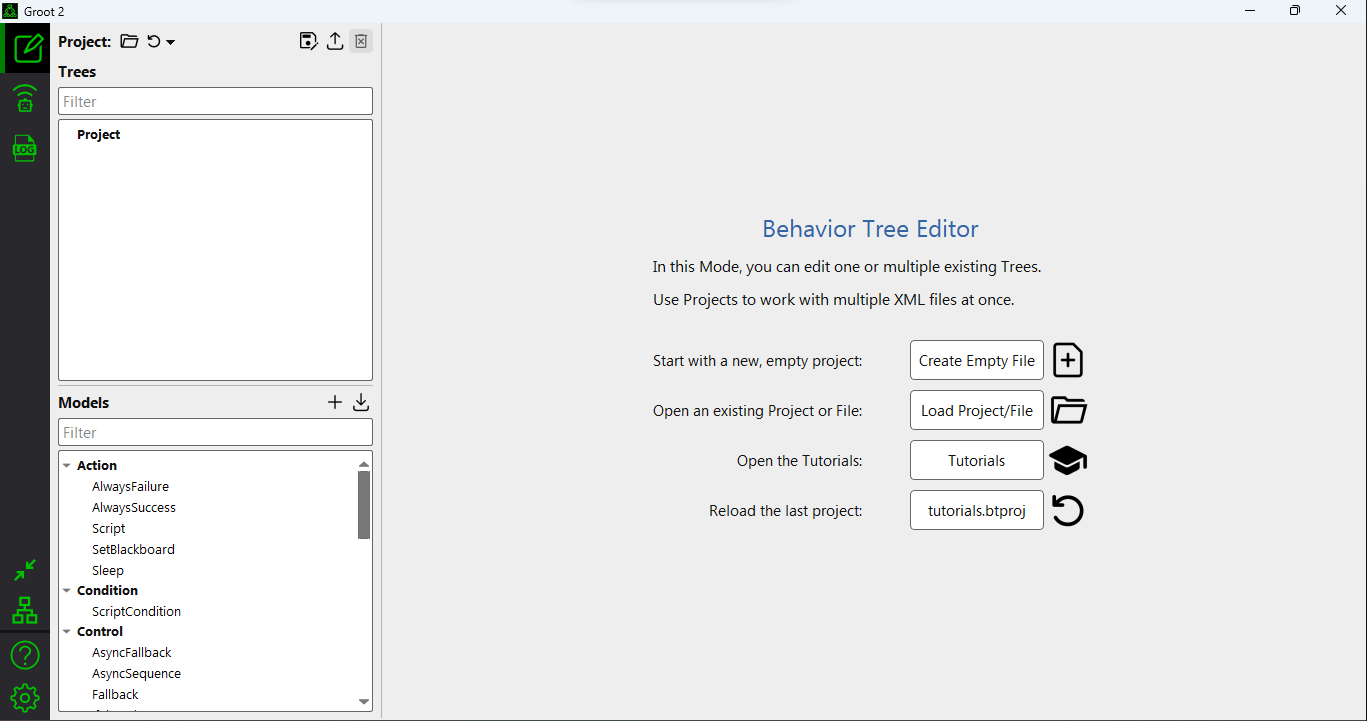
\includegraphics[width=1\textwidth]{images/groot2_start.png}
    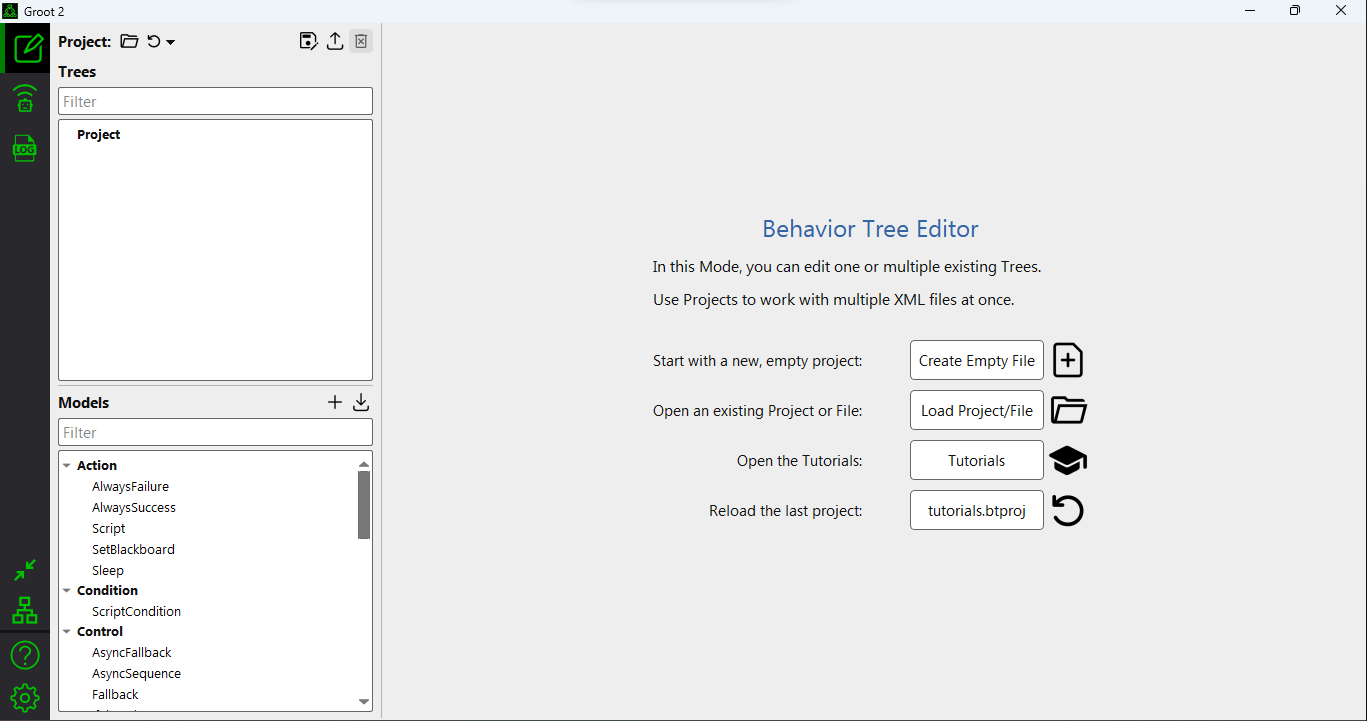
\includegraphics[width=120mm]{images/groot2_start.png}
    \caption{Groot2 IDE start screen}
    \label{fig:groo2_start}
\end{figure}

%%\newpage
%%\subsubsection{Groot2 Usage: Designing a simple behavior tree}
The Groot2 IDE (see Fig. \ref{fig:groo2_start}) is an essential tool for developing robot mission specifications within the CSSR4Africa software ecosystem, as it streamlines the process of creating and modifying behavior trees. 

To illustrate how Groot2 can be used to design a robot mission specification by implementing behavior trees, we can use a simple scenario example. In this example, a robot is tasked with picking and placing a ball. The mission is broken down into individual tasks, such as locating the ball, picking it up, moving it, and finally placing it at a designated spot. The final behavior tree that will be rcreated in Groot2 is shown in Fig. \ref{fig:pick_place_tree}.


\begin{figure}[htbp]
    \centering
    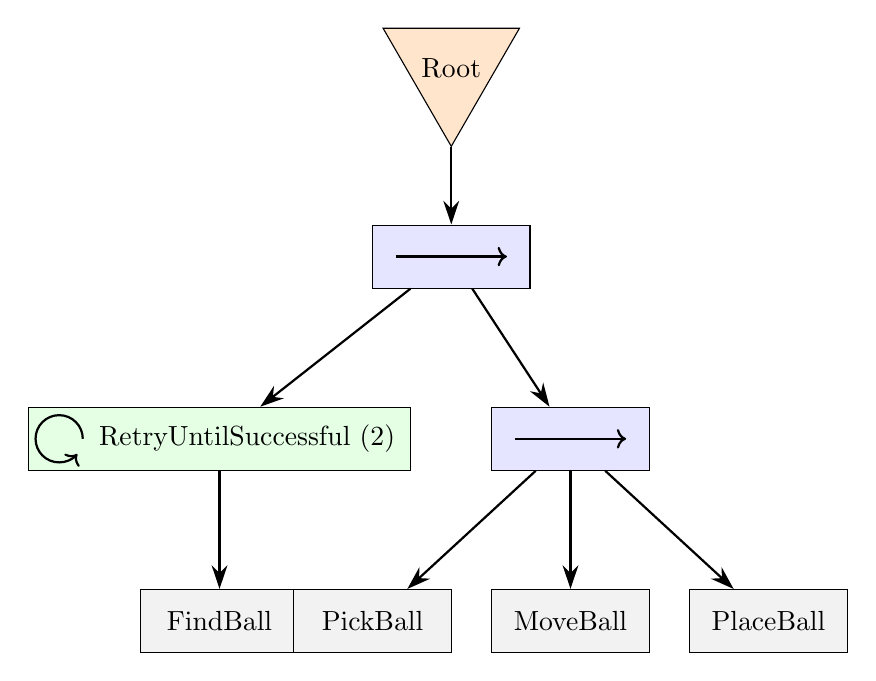
\begin{tikzpicture}[
        action/.style={draw, rectangle, minimum width=2cm, minimum height=0.8cm, align=center, inner sep=2mm, fill=gray!10},
        sequence/.style={draw, rectangle, minimum width=2cm, minimum height=0.8cm, align=center, inner sep=2mm, fill=blue!10},
        retry/.style={draw, rectangle, minimum width=2.5cm, minimum height=0.8cm, align=center, inner sep=2mm, fill=green!10},
        arrow/.style={-{Stealth[length=3mm, width=2mm]}, thick},
        level distance=1.5cm,
        sibling distance=3cm
      ]
      
      \node[draw, shape=regular polygon, regular polygon sides=3, rotate=180, minimum size=2cm, fill=orange!20] (rootshape) {};
      \node at (rootshape.center) {Root};
      
      \node[sequence, below=2.5cm of rootshape] (outerseq) {\hspace{0.1cm}};
      \begin{scope}[shift={($(outerseq.west) + (0.45cm,0)$)}]
      \draw[->, thick] ($(outerseq.west)+(0.3,0)$) -- ($(outerseq.east)+(-0.3,0)$);
      \end{scope}
      
      % RetryUntilSuccessful node
      \node[retry, below left=1.5cm and -0.5cm of outerseq] (retry) {\hspace{0.7cm}RetryUntilSuccessful (2)};
      \begin{scope}[shift={($(retry.west) + (0.6cm,0)$)}]
        \draw[->, thick] (0:0.1cm) arc (0:320:0.3cm);
      \end{scope}
      
      % FindBall node
      \node[action, below=1.5cm of retry] (findball) {FindBall};
      
      % Inner Sequence node
      \node[sequence, below right=1.5cm and -0.5cm of outerseq] (innerseq) {\hspace{0.1cm}};
      \begin{scope}[shift={($(innerseq.west) + (0.45cm,0)$)}]
        \draw[->, thick] ($(innerseq.west)+(0.3,0)$) -- ($(innerseq.east)+(-0.3,0)$);
      \end{scope}

      
      
      % Inner sequence nodes
      \node[action, below left=1.5cm and 0.5cm of innerseq] (pickball) {PickBall};
      \node[action, below=1.5cm of innerseq] (moveball) {MoveBall};
      \node[action, below right=1.5cm and 0.5cm of innerseq] (placeball) {PlaceBall};
      
      % edges
      \draw[arrow] (rootshape.north) -- (outerseq.north);
      \draw[arrow] (outerseq) -- (retry);
      \draw[arrow] (outerseq) -- (innerseq);
      \draw[arrow] (retry) -- (findball);
      \draw[arrow] (innerseq) -- (pickball);
      \draw[arrow] (innerseq) -- (moveball);
      \draw[arrow] (innerseq) -- (placeball);
      
      \end{tikzpicture}
    
    \caption{Behavior Tree for the Pick \& Place a Ball robot mission}
    \label{fig:pick_place_tree}
\end{figure}

%%The behavior tree is structured to execute the ``Pick \& Place Ball'' task as described above. It 
Under the root node, the behavior tree begins with a top-level \textbf{Sequence} node. This ensures that every step must succeed for the overall process to succeed. The first step involves a \textbf{RetryUntilSuccessful} decorator node that wraps the \textbf{FindBall} action node. This decorator attempts to locate the ball up to two times, allowing for a retry if the initial attempt fails; if the ball is not found after two attempts, the entire behavior tree fails. Once the ball is found, the tree proceeds to an inner \textbf{Sequence} node that orchestrates the subsequent actions. This node first executes the \textbf{PickBall} action to grasp the ball, then the \textbf{MoveBall} action node to transport it, and finally the \textbf{PlaceBall} action node to deposit it at the target location.


To begin, we open Groot2 and create a new tree file by clicking on the ``Create Empty File'' button. This will open a new window where we can design our behavior tree. The initial screen is shown in Fig. \ref{fig:groot2_new_tree}.
At this instance, there are no mission nodes defined yet. Only the control-flow nodes that are pre-defined by the IDE are available. So, we need to defined the three action nodes that we will use in our behavior tree. To that end, we click on the ``+'' button at the bottom left section, highlighted in red.


%\begin{figure}[H]
\begin{figure}[h]
    \centering
    %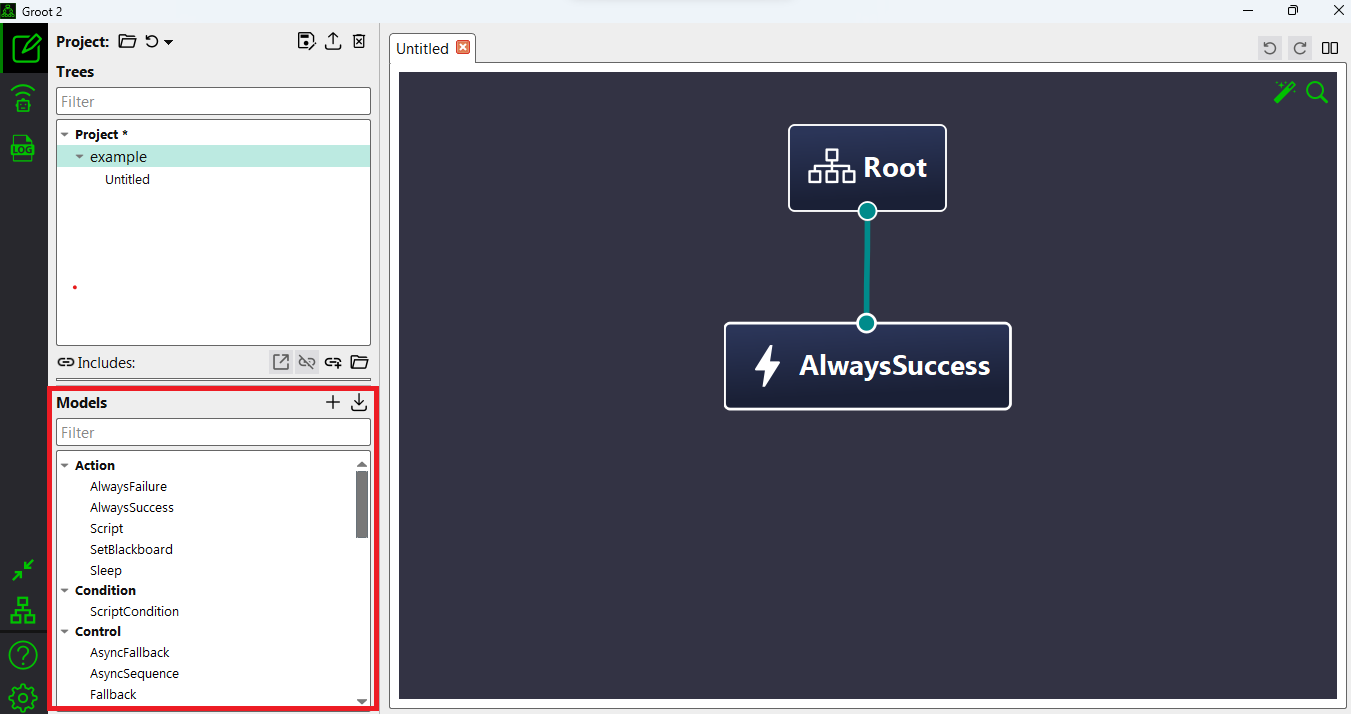
\includegraphics[width=\textwidth]{images/groot2_newtree.png}
    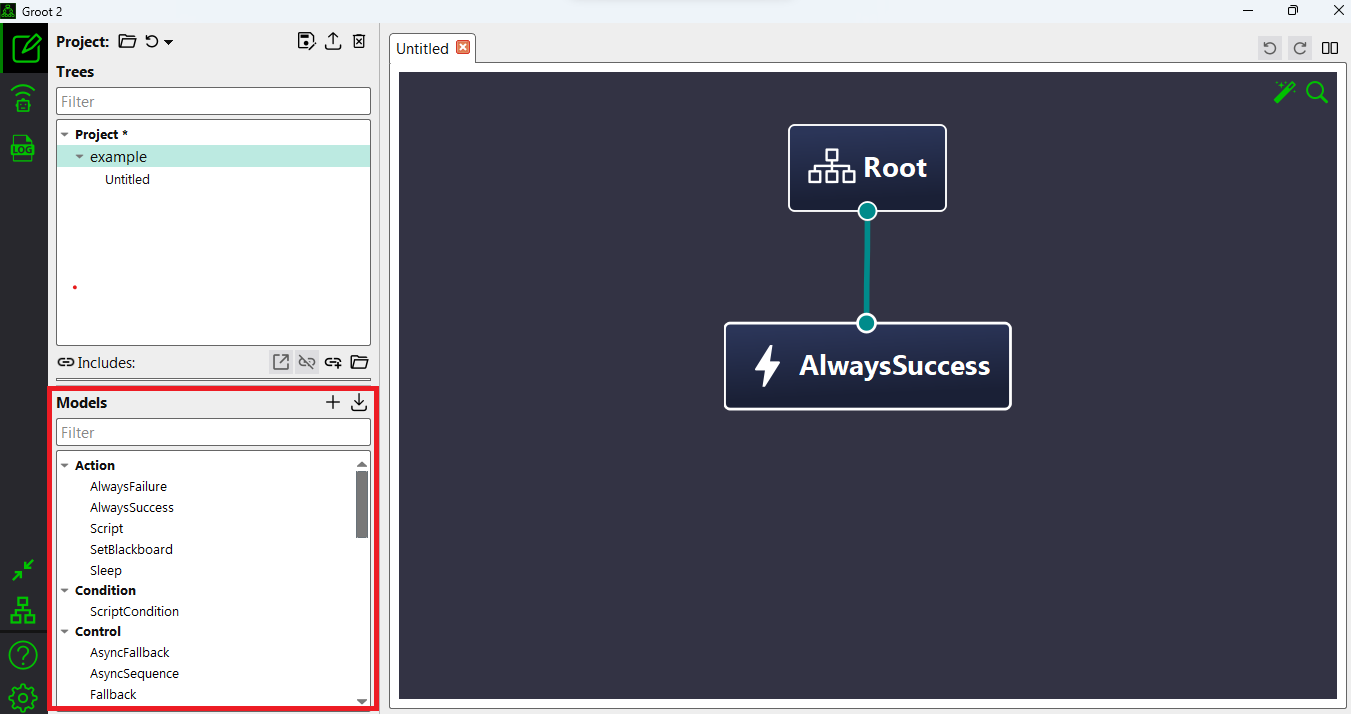
\includegraphics[width=120mm]{images/groot2_newtree.png}
    \caption{Groot2 New Tree Screen}
    \label{fig:groot2_new_tree}
\end{figure}



Once all the mission nodes are defined, they can be found under their specific category in the left panel, in this case ``Action''. We can drag and drop these nodes onto the canvas to create the behavior tree. These nodes are displayed in blue in Figure \ref{fig:groot2_nodesdefined}.


\begin{figure}[H]
    \centering
    %%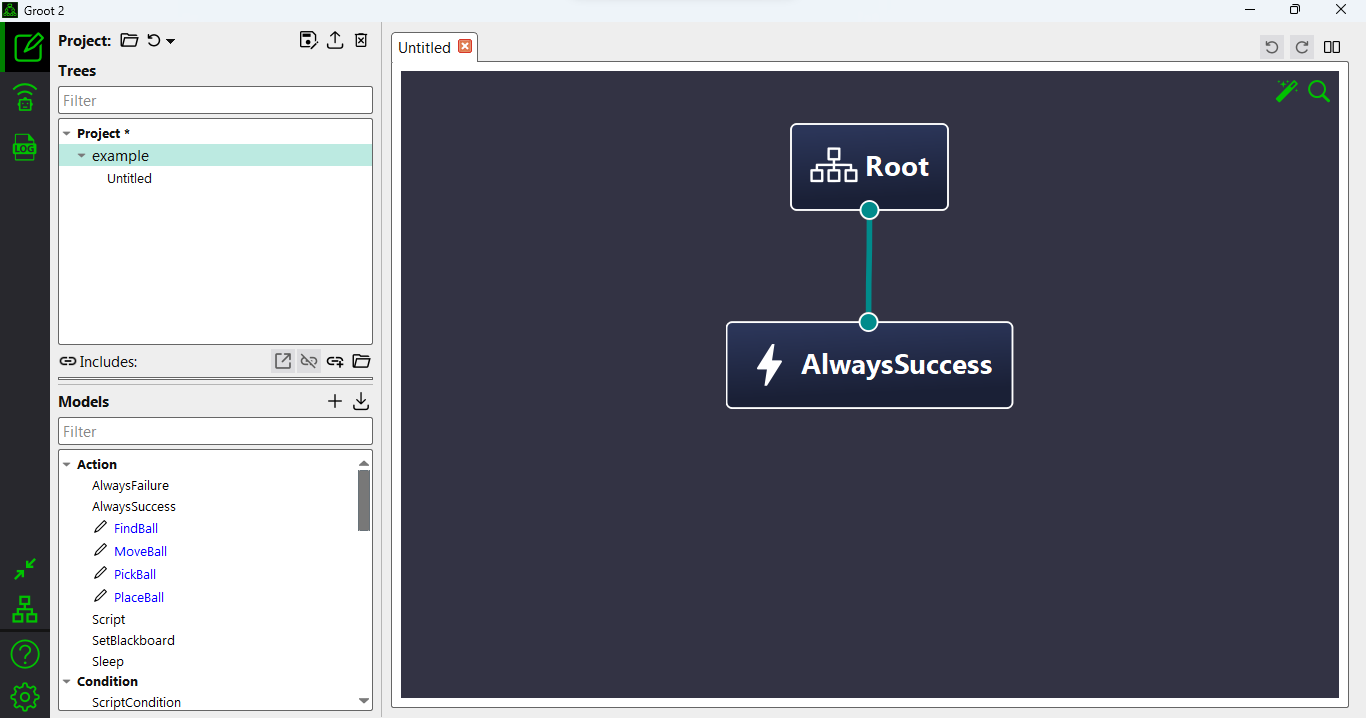
\includegraphics[width=1\textwidth]{images/groot2_nodesdefined.png}
    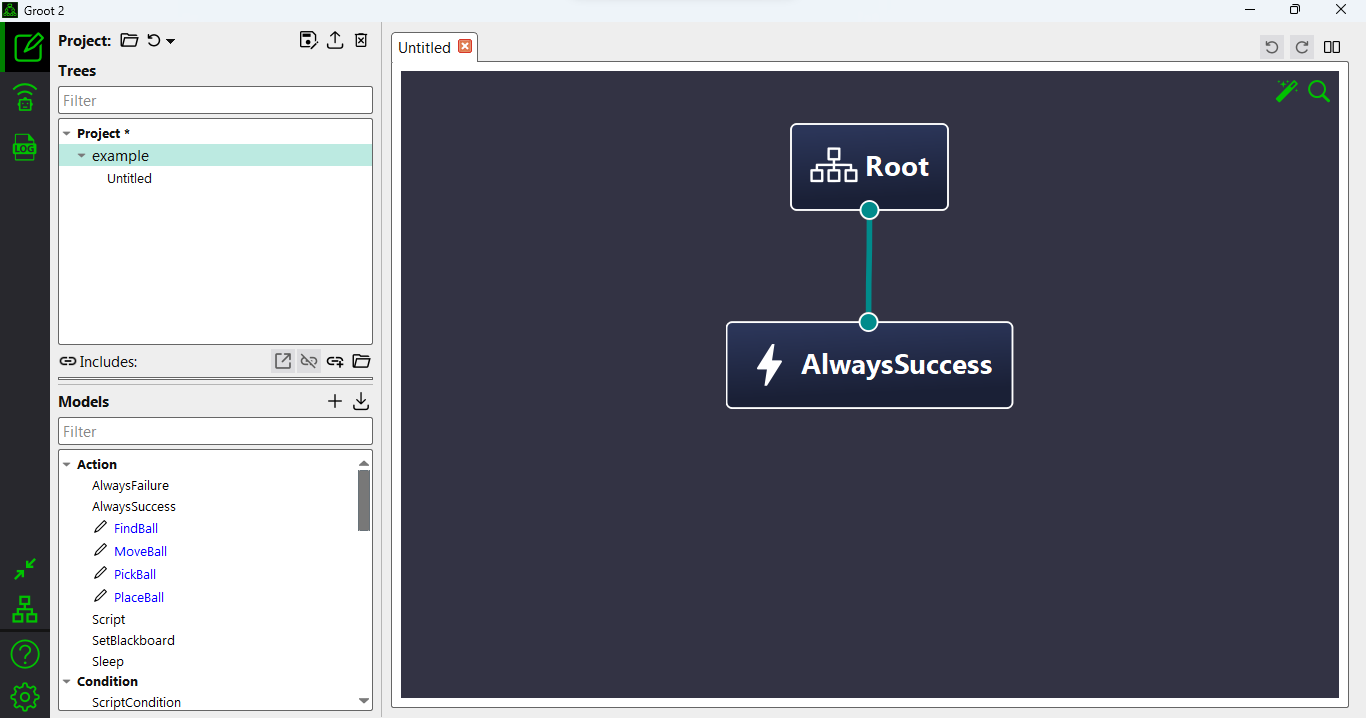
\includegraphics[width=120mm]{images/groot2_nodesdefined.png}
    \caption{Groot2 Actions Nodes Defined}
    \label{fig:groot2_nodesdefined}
\end{figure}


This will open a new window where we can define a new node; see Fig. \ref{fig:groo2_new_node}. We select the type of node we want to create from the drop-down menu. In this case, we select the \textbf{Action} node type. We then provide a name for the node, in this case, \textbf{FindBall}. 
We repeat this process for each action node in our behavior tree. 
%%The screen after defining the action nodes is shown in Fig. \ref{fig:groot2_nodesdefined}. 
%%\marginpar{\scriptsize \raggedright Is Fig. \ref{fig:groot2_nodesdefined} the correct figure? Shouldn't it be Fig. \ref{fig:groo2_tree_complete}. Also, isn't it premature to state this here, given the last sentence of the next paragraph?}

%\begin{figure}[H]
\begin{figure}[h]
    \centering
    %%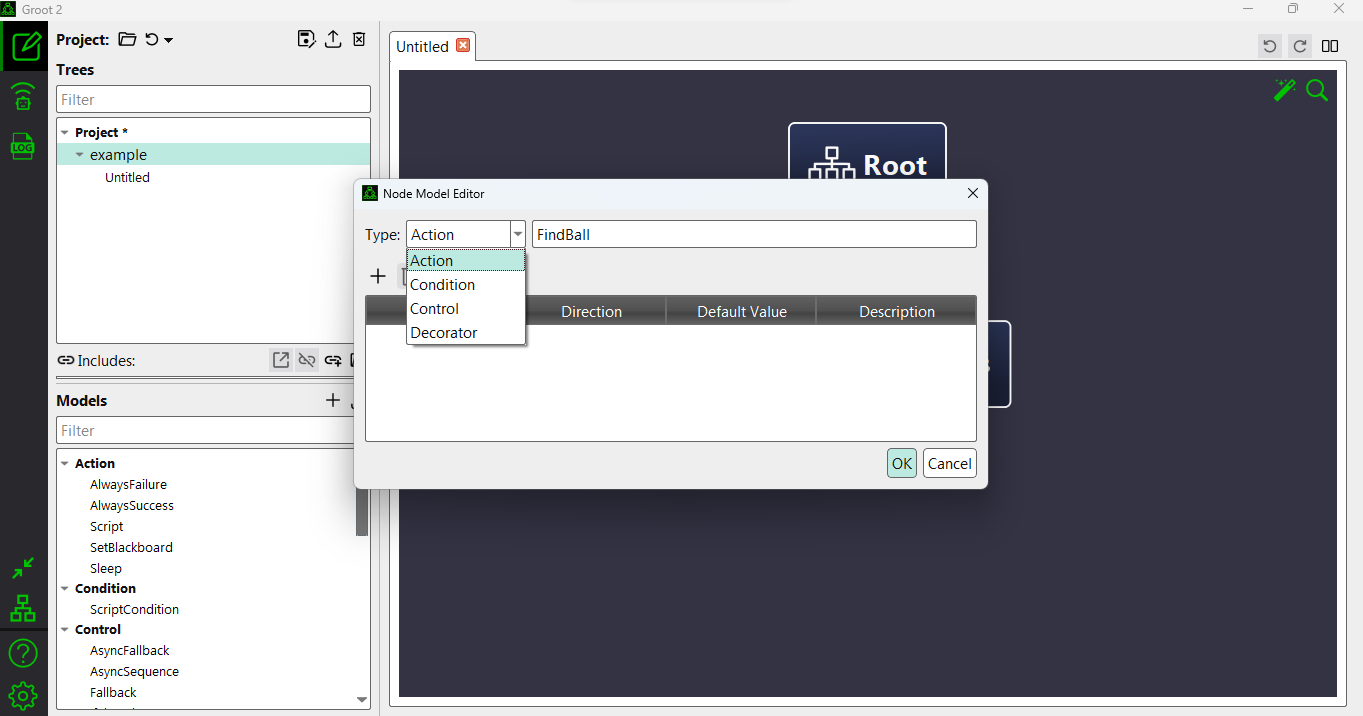
\includegraphics[width=\textwidth]{images/groot2_newnode.png}
    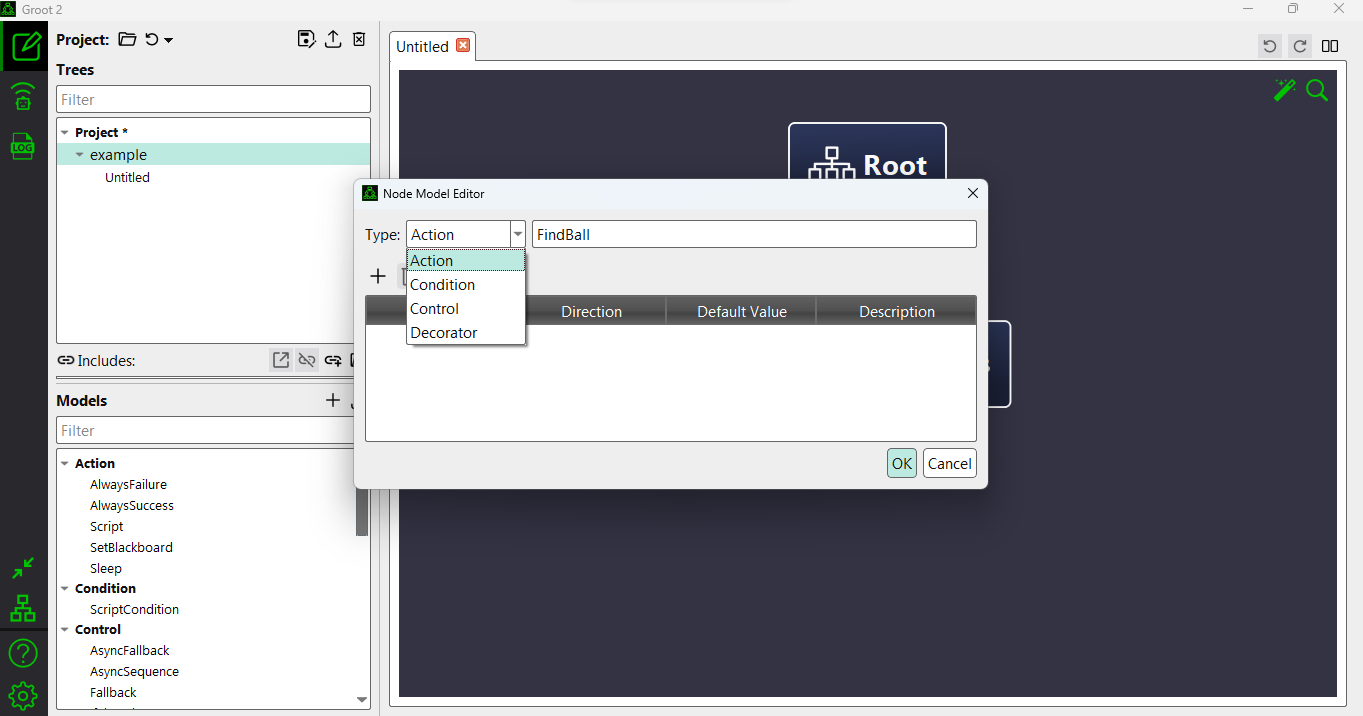
\includegraphics[width=120mm]{images/groot2_newnode.png}
    \caption{Groot2 New Node}
    \label{fig:groo2_new_node}
\end{figure}

Since our behavior tree starts with a \textbf{Sequence} node, we drag and drop a \textbf{Sequence} node from the left panel onto the canvas. Next, we add a \textbf{RetryUntilSuccessful} node by dragging it from the left panel and placing it under the \textbf{Sequence} node. Next, we add another \textbf{Sequence} node under the main \textbf{Sequence} node. We then add the \textbf{PickBall}, \textbf{MoveBall}, and \textbf{PlaceBall} action nodes under this inner \textbf{Sequence} node. The screen after adding these nodes is shown in Fig. \ref{fig:groo2_tree_complete}. 
\marginpar{\scriptsize }

\begin{figure}[H]
    \centering
    %%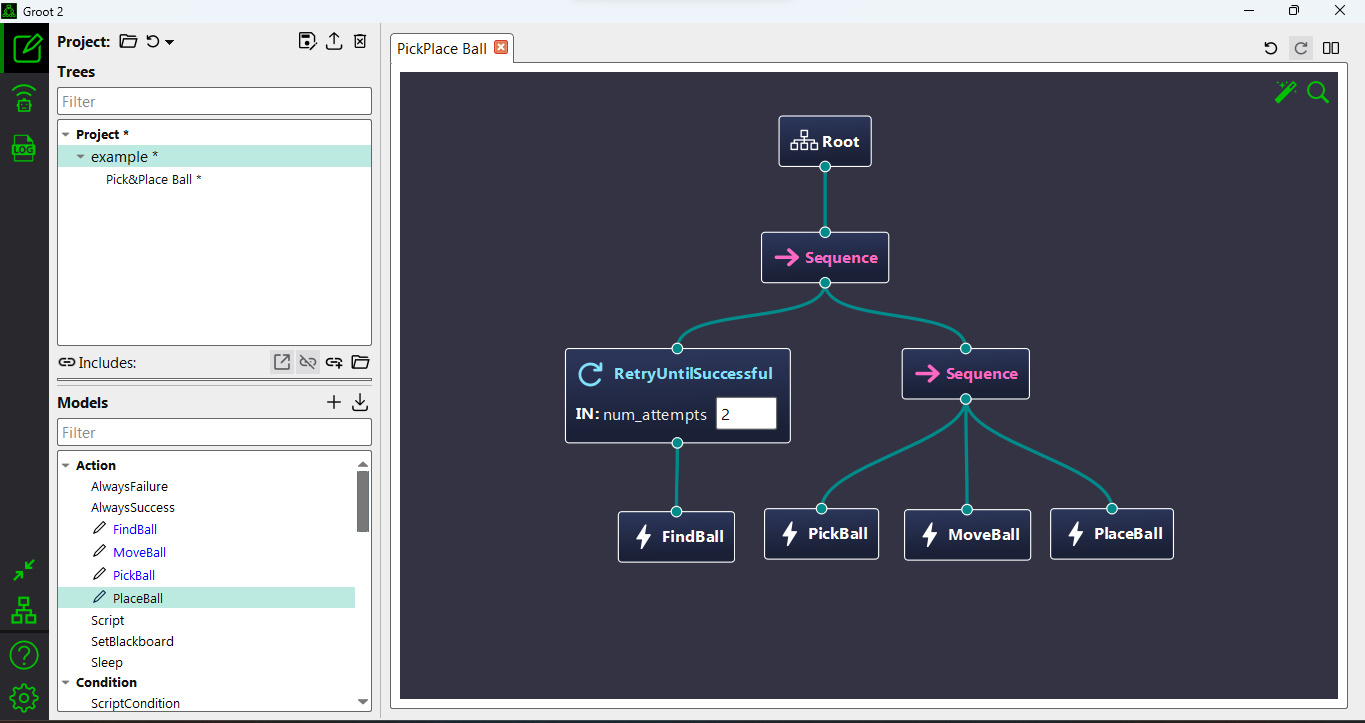
\includegraphics[width=1\textwidth]{images/groot2_tree_complete.png}
    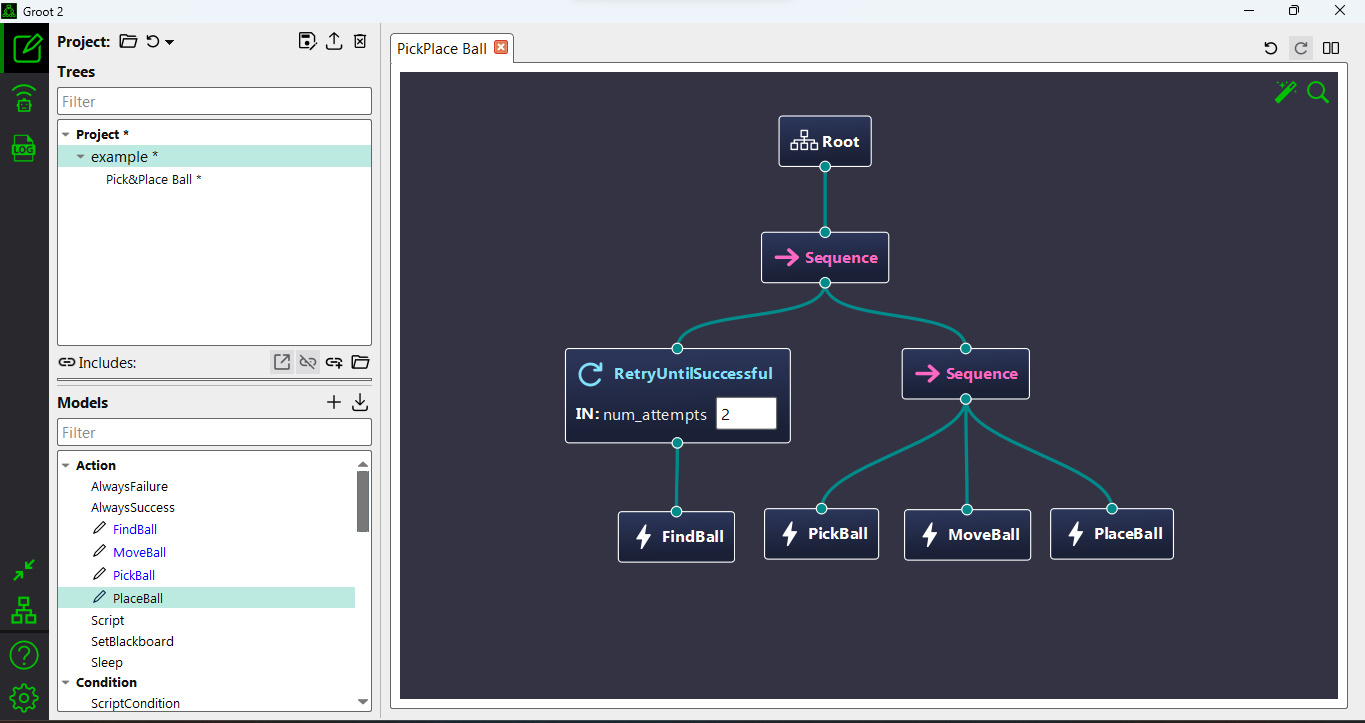
\includegraphics[width=120mm]{images/groot2_tree_complete.png}
    \caption{Groot2 Tree Complete}
    \label{fig:groo2_tree_complete}
\end{figure}

The behavior tree is now complete and ready for use. We can save the tree by clicking on the ``Save'' button at the top left corner of the screen. The tree can be exported in XML format by clicking on the ``Export'' button, represented by an arrow pointing upwards from a flat-line. The XML file can then be used in the robot mission interpreter to execute the specified mission.



\newpage

\section{Environment Knowledge Ontology and Knowledge Base}
%======================================
\label{section:knowledge_base}

Figure \ref{fig:knowledge_ontology} presents a simple ontology of environment knowledge.
In this ontology, internal nodes in the ontology tree form the key in the environment knowledge base, e.g., {\small \tt robotLocation}.  Leaf nodes represent the data entities and their types.  This allows  multiple elements in a value for each key, e.g., {\small \tt robotLocation 3 15.2 9.0 45.0}.  The identification number value element associated with each key is the means by which the different elements an environment location ---  robot location,  location description,  gesture target,  pre-gesture message,  post-gesture message --- are related.  The tour specification identifies the number and sequence of locations to be visited in the tour.


%\clearpage


Table \ref{table:key-value_pairs} lists the key-value pairs, i.e., each key and the associated multiple numeric or alphanumeric elements of the value that encapsulate the environment knowledge.  These numeric or alphanumeric values can then be used directly in the robot mission interpreter, i.e., the {\small \tt behaviorController} ROS node, and passed as arguments in the service requests it issues to the nodes in the system architecture to conduct a tour or provide directions as a response to an enquiry at reception.

The key-value pairs are stored in a file {\tt \small environmentKnowledgeBaseInput.dat}. This file is read and the value-pairs are accessed using a helper class {\tt \small EnvironmentKnowledgeBase} described in Section \ref{section:implementation}.  
 
\begin{table}[H]
\begin{center}
%%\vspace{-10mm}
\begin{tabular}{|l l l|}
\hline \hline
\multicolumn{3}{|c|}{{\small \bf Environment Knowledge}} \\
\hline \hline
 {\small Key  }                                                                          &  {\small Values }     &                               {\small Units }       \\
\hline
{\footnotesize \verb+robotLocationPose+} 	                          & {\footnotesize \verb+<IDNumber> <x> <y> <theta>+ } \vspace{0mm} & {\footnotesize Metres, degrees } \\
{\footnotesize \verb+robotLocationDescription+} 	                  & {\footnotesize \verb+<IDNumber> <text>+} \vspace{0mm} & {\footnotesize  String} \\
{\footnotesize \verb+gestureTarget+} 	                                  & {\footnotesize \verb+<IDNumber> <x> <y> <z>+} \vspace{0mm} & {\footnotesize  Metres} \\
{\footnotesize \verb+preGestureMessageEnglish+} 	           & {\footnotesize \verb+<IDNumber> <text>+} \vspace{0mm} & {\footnotesize  String } \\
{\footnotesize \verb+preGestureMessageIsizulu+} 	           & {\footnotesize \verb+<IDNumber> <text>+} \vspace{0mm} & {\footnotesize  String } \\
{\footnotesize \verb+preGestureMessageKinyarwanda+}         & {\footnotesize \verb+<IDNumber> <text>+} \vspace{0mm} & {\footnotesize  String } \\
{\footnotesize \verb+postGestureMessageEnglish+} 	           & {\footnotesize \verb+<IDNumber> <text>+} \vspace{0mm} & {\footnotesize  String} \\
{\footnotesize \verb+postGestureMessageIsizulu+} 	           & {\footnotesize \verb+<IDNumber> <text>+} \vspace{0mm} & {\footnotesize  String} \\
{\footnotesize \verb+postGestureMessageKinyarwanda+} 	   & {\footnotesize \verb+<IDNumber> <text>+} \vspace{0mm} & {\footnotesize  String} \\
{\footnotesize \verb+culturalKnowledge+} 	                          & {\footnotesize \verb+<IDNumber> <Key1>, <Key2>, ..., <Keyn>+} \vspace{0mm} & {\footnotesize  String} \\
{\footnotesize \verb+tourSpecification+} 	                        & {\footnotesize \verb+<n> <ID1>, <ID2>, ..., <IDn>+  } \vspace{0mm} & {\footnotesize  } \\
\hline \hline
\end{tabular}
\end{center}
\caption{Key-value pairs for specifying environment knowledge actions using the ontology depicted in Figure \ref{fig:knowledge_ontology}. As noted above, the identification number element of the value  associated with each key is the means by which the robot location, the location description, the gesture target, the pre-gesture message, the post-gesture message, and the cultural knowledge keys (from the cultural knowledge ontology) are related.  The tour specification identifies the number of locations and the sequence of locations to be visited in the tour. Note that the the angle {\tt \small <theta>} associated with the {\tt \small robotLocationPose} key must be a positive value. The need for this arises from problems using  literal value with a unary minus as an argument in rosservice calls. }
\label{table:key-value_pairs}
\end{table}


\begin{figure}[H]
%\vspace{-10 mm}
\dirtree{%
.1 Environment Knowledge.
.2 Robot Location.
.3 Identification Number (integer).
.3 Pose.
.4 x (float).
.4 y (float).
.4 theta (float).
.2 Robot Location Description.
.3 Identification Number (integer).
.3 Description (string).
.2 Gesture Target.
.3 Identification Number (integer).
.3 Position.
.4 x (float).
.4 y (float).
.4 z (float).
.2 Pre-gesture Message.
.3 Identification Number (integer).
.3 Description(string).
.4 English (string).
.4 Isizulu (string).
.4 Kinyarwanda (string).
.2 Post-gesture Message.
.3 Identification Number (integer).
.3 Description(string).
.4 English (string).
.4 Isizulu (string).
.4 Kinyarwanda (string).
.2 Cultural Knowledge (string).
.3 Identification Number (integer).
.3 Cultural Knowledge Key (string).
.3 Cultural Knowledge Key (string).
.3 … .
.3 Cultural Knowledge Key (string).
.2 Tour Specification.
.3 Number of Locations (integer).
.3 Location Sequence.
.4 Identification Number  (integer).
.4 Identification Number (integer).
.4 … .
.4 Identification Number (integer).
}
 
\caption{Environment knowledge ontology. }    
\label{fig:knowledge_ontology}
\end{figure}
 
\newpage
\section{Environment Knowledge Base Implementation}
%===============================================================
\label{section:implementation}

The key-value pairs listed in Tables \ref{table:key-value_pairs}, comprising an alphanumeric key and associated  numeric or symbolic values that encapsulate the environment knowledge, are stored in a file named\\ {\tt \small environmentKnowledgeBaseInput.dat}.  This file is accessed using a C++ helper class \\{\tt \small EnvironmentKnowledgeBase} described in this section.  Specifically, a C++ object instantiation of  the helper class  reads the environment knowledge base file, store the knowledge, and make the knowledge accessible through three public access methods. The remainder of this section details the implementation of this C++ helper class.
 

\subsection{File Organization}
%--------------------------

Since the C++ helper class is intended to be embedded in {\small \tt behaviorController} ROS node, it is not included as an individual component in the GitHub software repository.
That said, the constituent files are organized is several subdirectories in a {\small \tt utilities} package, as shown in Figure \ref{fig:directory_structure_utilities}. 

There are three C++ source code files:
{\small \tt environmentKnowledgeBaseApplication.cpp}, \\
{\small \tt environmenteKnowledgeBaseImplementation.cpp}, and 
{\small \tt environmentKnowledge.h}.  The implementation file contains the helper class definition. The interface file contains the helper class declaration. 

The application file is essentially a unit test to illustrate how the helper class is used and to verify that it works correctly. It instantiates a C++ helper class object which reads the environment knowledge base file, and uses the access method to retrieve  values in  the  environment knowledge base, implemented using a binary search tree dictionary data structure, write them to the terminal.

It is intended that the implementation and interface files, along with the configuration and data files, be integrated in the {\small \tt behaviorController} ROS node files.  The relevant parts of the {\small \tt behaviorController} software can use the application code as the basis of its implementation of functionality to access the knowledge base.


\begin{figure}[thb]
%%\vspace{20cm}
\dirtree{%
.1 utilities.
.2 config.
.3 environmentKnowledgeBaseConfiguration.ini.
.2 data.
.3 environmentKnowledgeBaseInput.dat.
.2 include.
.3 utilities.
.4 environmentKnowledgeBaseInterface.h.
.2 src.
.3 environmentKnowledgeBaseApplication.cpp.
.3 environmentKnowledgeBaseImplementation.cpp.
.2 launch.
.3 environmentKnowledgeBaseExample.launch.
.2 README.md.
.2 CMakeLists.txt.
}
\caption{Directory Structure for the {\tt \small EnvironmentKnowledgeBase}  C++ helper class.}
\label{fig:directory_structure_utilities}
\end{figure}


%\newpage

\subsection{Configuration File}
%--------------------------
The population of the knowledge base is determined by the contents of a configuration file
{\tt \small environmentKnowledgeBase.ini}  that  contain a list of key-value pairs, as shown below in Table~\ref{tab:config_file}.
The configuration file is named {\tt\small environmentKnowledgeBaseConfiguration.ini}.

 
%%\begin{longtable}[c]{|l|l|p{7cm}|}
\begin{table} [H]
\caption{Configuration file for the {\tt \small EnvironmentKnowledgeBase} helper class.} 
\label{tab:config_file}
\begin{tabularx}{\linewidth}{|l|l|X|}
    \hline
    \rowcolor{gray!30}
    \small{\textbf{Key}} & \small{\textbf{Value}} & \small{\textbf{Description}} \\ \hline
    %%\endhead % header for subsequent pages
    \footnotesize{\texttt{knowledgeBase}} & \footnotesize{\texttt{environmentKnowledgeBaseInput.dat}}  & \footnotesize{Specifies the filename of the file in which the cultural knowledge key-value pairs  are stored.} \\ \hline
    \footnotesize{\texttt{verboseMode}} & \footnotesize{\texttt{true}} or \texttt{false} & \footnotesize{Specifies whether diagnostic data is to be printed to the terminal.} \\ \hline
%%\end{longtable}
\end{tabularx}
\end{table}

\clearpage

\subsection{Environment Knowlege Base}
%------------------------
The environment knowledge base  file comprises a list of key-value pairs as shown in Table \ref{table:environmentKnowledgeBase}.  
 \lstdefinestyle{withoutNumbering}{
    backgroundcolor=\color{backcolour},   
    commentstyle=\color{black},
    keywordstyle=\color{black},
    stringstyle=\color{black},
    %%basicstyle=\ttfamily\small,
    basicstyle=\ttfamily\tiny,
    breakatwhitespace=false,         
    breaklines=true,                 
    captionpos=b,                    
    keepspaces=true,                 
    showspaces=false,                
    showstringspaces=false,
    showtabs=false,                  
    tabsize=2
}
\begin{table}[H]
%%\vspace{-5 mm}
\caption{Key-value pairs listed in the knowledge base file\\  {\tt \footnotesize environmentKnowledgeBaseInput.dat}.}
\label{table:environmentKnowledgeBase}
%\begin{center}
\vspace{0mm}
\begin{lstlisting}[style=withoutNumbering, language=bash]
robotLocationDescription       1 Pepper's starting location
robotLocationPose              1 2.6 8.1 270
gestureTarget                  1 0.0 0.0 0.0
preGestureMessageEnglish       1 Welcome the the robotics lab at Carnegie Mellon University Africa
preGestureMessageIsiZulu       1 No message in isiZulu
preGestureMessageKinyarwanda   1 Murakazaneza muri laboratwari ya robotikisi muri kaneji meloni iniverisite yafurika.
postGestureMessageEnglish      1 I will give you a short tour. I hope you enjoy it
postGestureMessageIsiZulu      1 No message in isiZulu
postGestureMessageKinyarwanda  1 Ngiye kubatemberezaho gato, nizereko muribuze kuryoherwa
CulturalKnowledge              1 SymbolicShapeRespect BowExtentRespect

robotLocationDescription       2 The (other) Pepper robot
robotLocationPose              2 2.6 8.1 315
gestureTarget                  2 3.2 8.4 0.82
preGestureMessageEnglish       2 This is the Pepper humanoid robot
preGestureMessageIsiZulu       2 No message in isiZulu
preGestureMessageKinyarwanda   2 Iyi yitwa pepa humanoyidi roboti
postGestureMessageEnglish      2 We use it for research in social robotics and human-robot interaction
postGestureMessageIsiZulu      2 No message in isiZulu
postGestureMessageKinyarwanda  2 Tuyikoresha mubushakashatsi mubijyanye nimibanire hamwe nimikoranire hagati yabantu
                                 ndetse naza robo
CulturalKnowledge              2 DeicticShape

robotLocationDescription       3 Lynxmotion
robotLocationPose              3 2.0 6.3 315
gestureTarget                  3 0.6 4.8 0.82
preGestureMessageEnglish       3 This is the Lynxmotion robot
preGestureMessageIsiZulu       3 No message in isiZulu
preGestureMessageKinyarwanda   3 Iyi robo ni likisi moshoni
postGestureMessageEnglish      3 We use it for teaching robot manipulation
postGestureMessageIsiZulu      3 No message in isiZulu
postGestureMessageKinyarwanda  3 Tuyikoresha mukwigisha roboti manipileshoni
CulturalKnowledge              3 DeicticShape

robotLocationDescription       4 Roomba
robotLocationPose              4 5.0 3.9 110
gestureTarget                  4 6.8 4.8 0.82
preGestureMessageEnglish       4 This is the Roomba
preGestureMessageIsiZulu       4 No message in isiZulu
preGestureMessageKinyarwanda   4 Iyiyo yitwa rumba
postGestureMessageenglish      4 We use it for teaching mobile robotics
postGestureMessageIsiZulu      4 No message in isiZulu
postGestureMessageKinyarwanda  4 Tuyikoresha mukwigisha mobile robotikisi
CulturalKnowledge              4 DeicticShape

robotLocationDescription       5 Pepper's starting location
robotLocationPose              5 2.6 8.1 270
gestureTarget                  5 0.0 0.0 0.0
preGestureMessageEnglish       5 I hope you enjoyed the tour
preGestureMessageIsiZulu       5 No message in isiZulu
preGestureMessageKinyarwanda   5 Nizereko mwaryohewe no gutemberezwa
postGestureMessageEnglish      5 See you again soon
postGestureMessageIsiZulu      5 No message in isiZulu
postGestureMessageKinyarwanda  5 Tuzongere kubonana ubutaha
CulturalKnowledge              5 IconicShape

tourSpecification 5 1 4 3 2 5

\end{lstlisting}
%\end{center}
\vspace{-5mm}
\end{table}
 

\subsection{Output Data File}
%------------------------
There is no output data file for the environment knowledge base helper class. 


\subsection{Class Definition}
%------------------------
Instantiating the {\tt\small EnvironmentKnowledgeBase} class as a C++ object causes the contents of the  environment knowledge base file to be read and stored in private  dictionary data structure. Diagnostic messages are printed on the screen, depending on the value of \texttt{verboseMode} key in the configuration file. The contents of the dictionary are accessed using the identification number. 
Appendix \ref{appendix:helper_class} provides the full definition of the {\tt\small EnvironmentKnowledgeBase} class.

\subsubsection{Constructor}
%--------------------------

The  {\tt\small EnvironmentKnowledgeBase()} constructor reads the configuration file to determine the mode of operation, the name of the knowledge base value types file, and  the name of the knowledge base file. It sets a private data member flag with the mode of operation, initializes the private dictionary data structure with the key-value pairs read from the knowledge base file. If operating in verbose mode, it echoes the keys and values to the terminal.


\subsubsection{Destructor}
%--------------------------

The  {\tt\small \verb+~+EnvironmentKnowledgeBase()} destructor deletes the dictionary data structure and write a diagnostic message if in verbose mode.


\subsubsection{Private Data}
%--------------------------

The dictionary is implemented using a binary search tree with an element of type {\small \tt struct KeyValueType}, with eleven fields.

 \lstdefinestyle{withoutNumbering}{
    backgroundcolor=\color{backcolour},   
    commentstyle=\color{black},
    keywordstyle=\color{black},
    stringstyle=\color{black},
    %%basicstyle=\ttfamily\scriptsize,
    basicstyle=\ttfamily\tiny,
    breakatwhitespace=false,         
    breaklines=true,                 
    captionpos=b,                    
    keepspaces=true,                 
    showspaces=false,                
    showstringspaces=false,
    showtabs=false,                  
    tabsize=2
}
\begin{lstlisting}[style=withoutNumbering, language=bash]
typedef struct {
   float x;
   float y;
   float theta;
} RobotLocationType;

typedef struct {
   int numberOfKeys;
   char *key[MAX_CULTURAL_KEYS];
} CulturalKnowledgeType;

typedef struct {
   float x;
   float y;
   float z;
} GestureTargetType;

typedef  struct {
    int                   key; // location identification number
    RobotLocationType     robotLocation;
    char                  robotLocationDescription[STRING_LENGTH];
    GestureTargetType     gestureTarget;
    CulturalKnowledgeType culturalKnowledge;
    char                  preGestureMessageEnglish[STRING_LENGTH];
    char                  preGestureMessageIsiZulu[STRING_LENGTH];
    char                  preGestureMessageKinyarwanda[STRING_LENGTH];
    char                  postGestureMessageEnglish[STRING_LENGTH];
    char                  postGestureMessageIsiZuluSTRING_LENGTH];
    char                  postGestureMessageKinyarwanda[STRING_LENGTH];
} KeyValueType;
 
\end{lstlisting}
\noindent
The first field {\small \tt key} is the identification number for this location. The data type is integer. This is the key that is used to access data in the binary search tree dictionary.
\\~\\
The second field {\small \tt robotLocation} is a structure with three members containing the $x$, $y$, and $\theta$ floating point values that specify the pose of the robot at this location. 
\\~\\
The third field {\small \tt robotLocationDescription} is a description of this robot location.  The data type  is a C-string, i.e., a null-terminated array of characters.
\\~\\
The fourth field {\small \tt gestureTarget} is a structure with three members containing the $x$, $y$, and $z$ floating point values that specify the position of the target to which the robot is to gesture.  
\\~\\
The fifth field {\small \tt culturalKnowledge} is a structure with two members, one specifying the number of keys in the cultural knowledge bases that are associated with this location, and the other listing them.  These keys can then be used to look up the associated value in the culture knowledge base. At present, the data structure can store a maximum of ten keys. This can be adjusted by changing the value of the {\small \verb+#define MAX_CULTURAL_KEYS+} constant.
\\~\\
The  sixth, seventh, and eighth fields are messages to be spoken by the robot prior to executing the gesture; there are three versions, one in English, one in isiZulu, and one in Kinyarwanda. The data type  is a C-string, i.e., a null-terminated array of characters.
\\~\\
The  ninth,  tenth, and eleventh fields are messages to be spoken by the robot after executing the gesture; again, there are three versions, one in English, one in isiZulu, and one in Kinyarwanda. The data type  is a C-string, i.e., a null-terminated array of characters.
\\~\\
In addition to the binary search tree dictionary data structure, there is also a data structure\\ {\small \tt tourSpecification} to specify the tour. This is a structure with two members: an integer specifying the number of robot locations in a tour and an array of  integer identification numbers specifying sequence of robot locations  that the robot should visit during the tour, in the order in which they are stored in the array.

 \lstdefinestyle{withoutNumbering}{
    backgroundcolor=\color{backcolour},   
    commentstyle=\color{black},
    keywordstyle=\color{black},
    stringstyle=\color{black},
    basicstyle=\ttfamily\scriptsize,
    %%basicstyle=\ttfamily\tiny,
    breakatwhitespace=false,         
    breaklines=true,                 
    captionpos=b,                    
    keepspaces=true,                 
    showspaces=false,                
    showstringspaces=false,
    showtabs=false,                  
    tabsize=2
}
\begin{lstlisting}[style=withoutNumbering, language=bash]
typedef struct {
   int numberOfLocations;
   int locationIdNumber[MAX_NUMBER_OF_TOUR_LOCATIONS];
} TourSpecificationType;

\end{lstlisting}

\noindent
There are also a small number of other private utility data fields to store the configuration filename, the configuration data, a keyValue, and the verbose mode flag.


\newpage
\subsubsection{Public Access Methods}
%----------------------------------
There are three public methods, one to print the knowledge base to the screen,  one to retrieve a key-value pair, given the identification number of the  location, and one to retrieve the tour specification. These are {\small \tt printToScreen()},  {\small \tt getValue()}, and  {\small \tt getTour()}, respectively.
~\\~\\
The {\small \tt printToScreen()} method does not have any parameters.
~\\~\\
The  {\small \tt getValue()}  method has two parameters: a key and a value, as follows.

\begin{lstlisting}[style=withoutNumbering, language=bash] 
bool getValue(int idNumber, KeyValueType *keyValue);
\end{lstlisting}

\noindent The method returns {\small \tt true} if the key value was successfully retrieved from the knowledge base, {\small \tt false} otherwise.
~\\~\\
The  {\small \tt getTour()}  method has one parameter: the tour data, as follows.

\begin{lstlisting}[style=withoutNumbering, language=bash] 
bool getTour(struct TourSpecificationType *tourSpecification);
\end{lstlisting}

\noindent The method returns {\small \tt true} if the  tour was successfully retrieved from the knowledge base, {\small \tt false} otherwise.


 \newpage
\section{Example Application}
%===============================================================
\label{section:application}
%\vspace{-3mm}
The example application in {\small \tt environmentKnowledgeBaseApplication.cpp} illustrates the use of the class to read the environment knowledge base file and print each key-value pair with multiple elements.  It also provides examples of how to retrieve the values associated with a robot location given by its identification number, and how to retrieve the sequence of robot locations in a tour. \\
\vspace{-5mm}
\lstdefinestyle{withoutNumbering}{
    backgroundcolor=\color{backcolour},   
    commentstyle=\color{black},
    keywordstyle=\color{black},
    stringstyle=\color{black},
    %%basicstyle=\ttfamily\small,
    basicstyle=\ttfamily\scriptsize,
    basicstyle=\ttfamily\tiny,
    breakatwhitespace=false,         
    breaklines=true,                 
    captionpos=b,                    
    keepspaces=true,                 
    showspaces=false,                
    showstringspaces=false,
    showtabs=false,                  
    tabsize=2
}
\begin{lstlisting}[style=withoutNumbering, language=bash]
#include <utilities/environmentKnowledgeBaseInterface.h>

int main() {
   KeyValueType          keyValue; // structure with key and values
   TourSpecificationType tour;     // list of tour locations
   int                   idNumber; // location id
   int                   i;        // counter
   int                   k;        // counter

   /* instantiate the environment knowledge base object                      */
   /* this reads the knowledge value types file and the knowledge base file  */
   /* as specified in the environmentKnowledgeBaseConfiguration.ini file     */
  
   EnvironmentKnowledgeBase knowledgebase;  

   /* verify that the knowledge base was read correctly */

   printf("main: the environment knowledge base data:\n");
   printf("------------------------------------------\n\n");
   
   knowledgebase.printToScreen();

   printf("main: the environment knowledge base tour:\n");
   printf("-----------------------------------------\n\n");

   knowledgebase.getTour(&tour);
  
   /* query the contents of the knowledge base:               */
   /* retrieve all the locations on a tour                    */
   /* and print them in the order in which they are specified */

   for (i = 0; i <= tour.numberOfLocations; i++) {
      idNumber = tour.locationIdNumber[i];
      if (knowledgebase.getValue(idNumber, &keyValue) == true) {
         printf("main:\n"
         "Key                              %-4d \n"
         "Location Description             %s \n"
         "Robot Location                   (%.1f, %.1f  %.1f)\n"
         "Gesture Target                   (%.1f, %.1f  %.1f) \n"
         "Pre-Gesture Message English      %s \n"
         "Pre-Gesture Message isiZulu      %s \n"
         "Pre-Gesture Message Kinyarwanda  %s \n"
         "Post-Gesture Message             %s \n"
         "Post-Gesture Message isiZulu     %s \n"
         "Post-Gesture Message Kinyarwanda %s \n",
         keyValue.key,
         keyValue.robotLocationDescription, 
         keyValue.robotLocation.x, keyValue.robotLocation.y, keyValue.robotLocation.theta,
         keyValue.gestureTarget.x, keyValue.gestureTarget.y, keyValue.gestureTarget.z,
         keyValue.preGestureMessageEnglish,
         keyValue.preGestureMessageIsiZulu,
         keyValue.preGestureMessageKinyarwanda,
         keyValue.postGestureMessageEnglish,
         keyValue.postGestureMessageIsiZulu,
         keyValue.postGestureMessageKinyarwanda);

         printf("Cultural Knowledge                ");
         for (k=0; k<keyValue.culturalKnowledge.numberOfKeys; k++) {
            printf("%s ", keyValue.culturalKnowledge.key[k]);
      }

         printf("\n\n");
   }
}
}
\end{lstlisting}
\noindent
Run the application by entering the following command:
\lstdefinestyle{withoutNumbering}{
    backgroundcolor=\color{backcolour},   
    commentstyle=\color{codegreen},
    keywordstyle=\color{magenta},
    stringstyle=\color{codepurple},
    %%basicstyle=\ttfamily\small,
    basicstyle=\ttfamily\footnotesize,
    breakatwhitespace=false,         
    breaklines=true,                 
    captionpos=b,                    
    keepspaces=true,                 
    showspaces=false,                
    showstringspaces=false,
    showtabs=false,                  
    tabsize=2
}
\begin{lstlisting}[style=withoutNumbering, language=bash]
rosrun utilities environmentKnowledgeBaseExample
\end{lstlisting}
This assumes the existence of a {\small \tt utilities} package, as shown in Figure  \ref{fig:directory_structure_utilities}, and that the package has been built with {\small \tt catkin\_make}. \\~\\
Screenshots of the output of running this application are shown in Figures \ref{fig:screenshot1} and \ref{fig:screenshot2}.
 
\newpage
\begin{figure}[H]
\begin{center}
\vspace{-2mm}
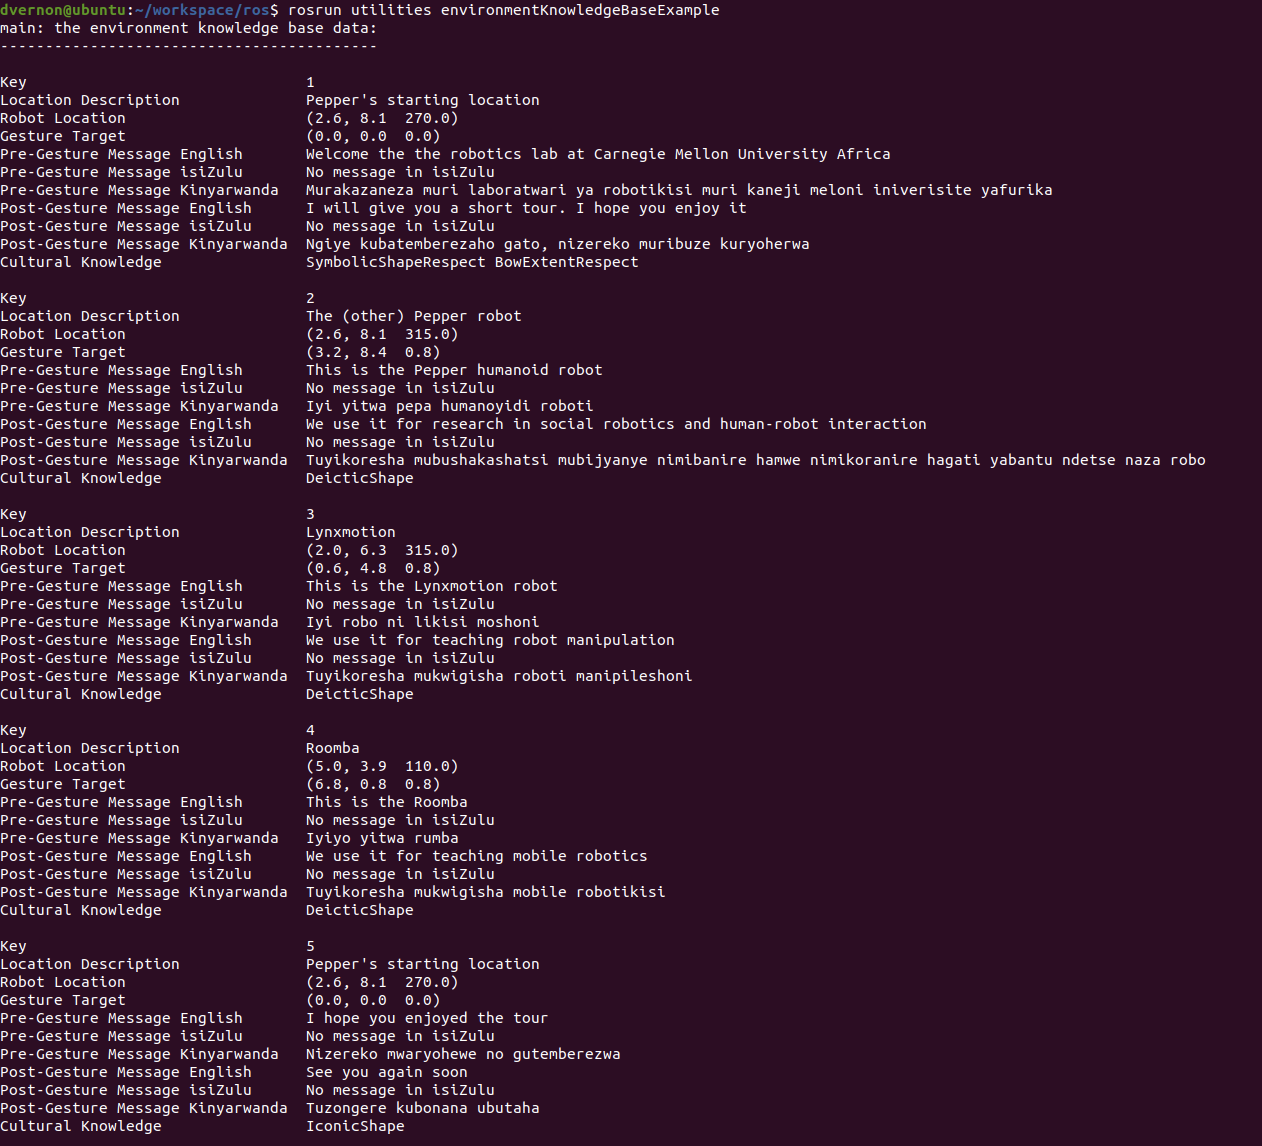
\includegraphics[width=\linewidth,angle=0]{screenshot1.png}
\end{center}
\vspace{-6mm}
\caption{Screenshot of  the output of running the example  application: invoking {\small \tt printToScreen()}.}
\label{fig:screenshot1}       
\end{figure}

\begin{figure}[H]
\begin{center}
\vspace{-5mm}
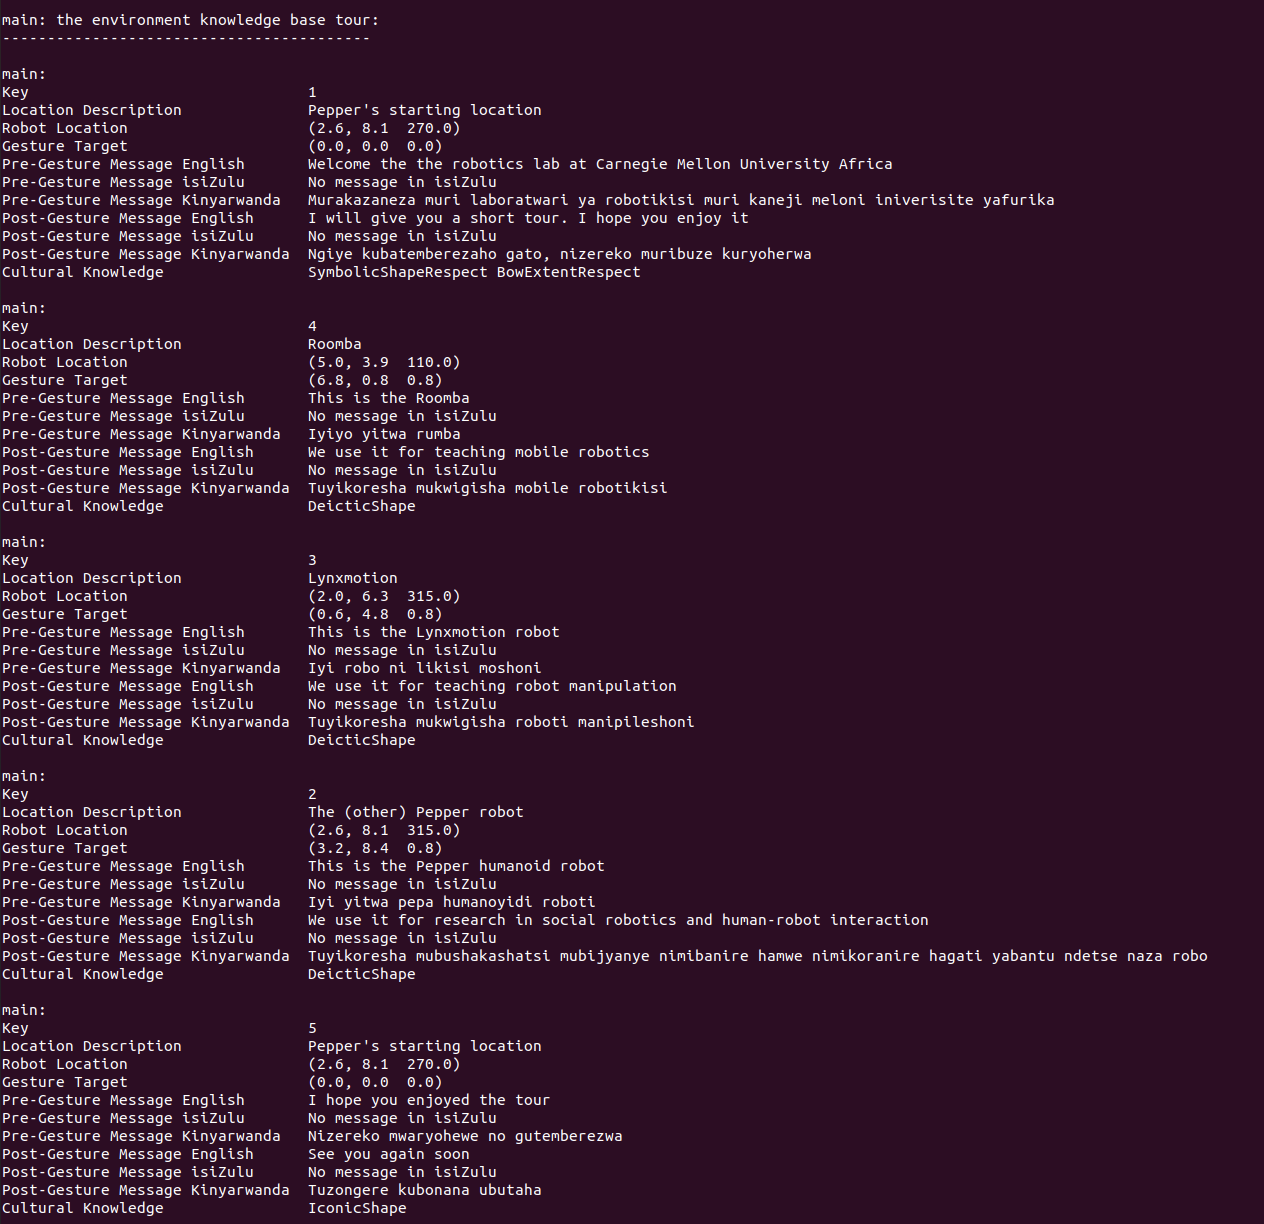
\includegraphics[width=\linewidth,angle=0]{screenshot2.png}
\end{center}
\vspace{-6mm}
\caption{Screenshot of  the output of running the example  application:  invoking {\small \tt getTour()} and invoking {\small \tt getValue()} successively for each location on the tour.}
\label{fig:screenshot2}       
\end{figure}


\newpage
\begin{appendices}
%###############################################################################
~
\vspace{-15mm}
%===============================================================
\section{The EnvironmentKnowledgeBase Class}
%===============================================================
\label{appendix:helper_class}  
\vspace{-2mm}
Note: documentation comments for the private methods have been removed due to space constraints.

\lstdefinestyle{withoutNumbering}{
    backgroundcolor=\color{backcolour},   
    commentstyle=\color{black},
    keywordstyle=\color{magenta},
    stringstyle=\color{black},
    %%basicstyle=\ttfamily\small,
    basicstyle=\ttfamily\tiny,
    breakatwhitespace=false,         
    breaklines=true,                 
    captionpos=b,                    
    keepspaces=true,                 
    showspaces=false,                
    showstringspaces=false,
    showtabs=false,                  
    tabsize=2
}
\begin{lstlisting}[style=withoutNumbering, language=bash]
#define NUMBER_OF_CONFIGURATION_KEYS  2
#define NUMBER_OF_VALUE_KEYS         11
#define MAX_NUMBER_OF_TOUR_LOCATIONS 20
#define MAX_CULTURAL_KEYS            10

typedef char Keyword[KEY_LENGTH];

typedef struct {
   char knowledgeBase[MAX_FILENAME_LENGTH];
   bool verboseMode;
} ConfigurationDataType;

typedef struct {
   float x;
   float y;
   float theta;
} RobotLocationType;

typedef struct {
   int numberOfKeys;
   char *key[MAX_CULTURAL_KEYS];
} CulturalKnowledgeType;

typedef struct {
   float x;
   float y;
   float z;
} GestureTargetType;

typedef struct {
   int numberOfLocations;
   int locationIdNumber[MAX_NUMBER_OF_TOUR_LOCATIONS];
} TourSpecificationType;

typedef  struct {
    int                   key; // i.e., idNumber
    RobotLocationType     robotLocation;
    char                  robotLocationDescription[STRING_LENGTH];
    GestureTargetType     gestureTarget;
    CulturalKnowledgeType culturalKnowledge;
    char                  preGestureMessageEnglish[STRING_LENGTH];
    char                  preGestureMessageIsiZulu[STRING_LENGTH];
    char                  preGestureMessageKinyarwanda[STRING_LENGTH];
    char                  postGestureMessageEnglish[STRING_LENGTH];
    char                  postGestureMessageIsiZuluSTRING_LENGTH];
    char                  postGestureMessageKinyarwanda[STRING_LENGTH];
} KeyValueType;

typedef struct node *NodeType;

typedef struct node {
            KeyValueType keyValue;
            NodeType left, right;
         } Node;

typedef NodeType BinaryTreeType;

typedef BinaryTreeType WindowType;

class EnvironmentKnowledgeBase {

public:
   EnvironmentKnowledgeBase();
   ~EnvironmentKnowledgeBase();
   
   bool                  getValue(int key, KeyValueType *keyValue);   
   bool                  getTour(TourSpecificationType  *tour);     
   void                  printToScreen();                                      

private:
   BinaryTreeType        tree = NULL; 
   TourSpecificationType tourSpecification;
   KeyValueType          keyValue;
   ConfigurationDataType configurationData;
   char                  configuration_filename[MAX_STRING_LENGTH] = "environmentKnowledgeBaseConfiguration.ini";


   BinaryTreeType        *delete_element(KeyValueType keyValue, BinaryTreeType *tree);  
   KeyValueType          delete_min(BinaryTreeType *tree); 
   bool                  getValue(int key, KeyValueType *keyValue, BinaryTreeType *tree);   
   void                  initialize(BinaryTreeType *tree);                    
   int                   inorder_print_to_file(BinaryTreeType tree, int n, FILE *fp_out);    
   int                   inorder_print_to_screen(BinaryTreeType tree, int n);           
   BinaryTreeType        *insert(KeyValueType keyValue, BinaryTreeType *tree, bool update);   
   int                   postorder_delete_nodes(BinaryTreeType tree);      
   int                   print_to_file(FILE *fp_out);              
   int                   print_to_file(BinaryTreeType tree, FILE *fp_out);        
   int                   print_to_screen(BinaryTreeType tree);    
   void                  readConfigurationData();  
   void                  readKnowledgeBase();     
};


\end{lstlisting}

 \end{appendices}
%###############################################################################



\newpage
\bibliographystyle{unsrt}
%================================================================
\bibliography{cognitive_systems.bib}   
%%\bibliography{../../../DV_Publications/bibliography/cognitive_systems.bib}                                                                     
\addcontentsline{toc}{section}{References}

 

\pagebreak
\section*{Principal Contributors}
%===============================================================
\label{contributors}
\addcontentsline{toc}{section}{Principal Contributors}
The main authors of this deliverable are as follows (in alphabetical order).
\blank
~
\blank
Clifford Oyononka, Carnegie Mellon University Africa.\\
Tsegazeab Tefferi, Carnegie Mellon University Africa.\\    
David Vernon, Carnegie Mellon University Africa.\\   
  

\newpage
\section*{Document History}
%================================================================
\addcontentsline{toc}{section}{Document History}
\label{document_history}

\begin{description}

\item [Version 1.0]~\\
Partial version to address the specification of the environment knowledge base and \\{\small \tt EnvironmentKnowledgeBase} helper class. \\
David Vernon.\\
5 March 2025.                                            


\item [Version 1.1]~\\
Removed  the {\small \tt utilities} sub-directory since the C++ helper classes will be integrated directly in the software for the {\small \tt behaviorController} node and not be made available independently.\\
Extended the ontology and added new keys to allow for pre- and post-gesture messages in English, isiZulu, and Kinyarwanda.\\
David Vernon.\\
11 March 2025.     


\item [Version 1.2]~\\
Updated the ontology to rectify the duplicate robot location internal nodes, changing the second to robot location description.\\
Changed the robotLocation key to robotLocationPose in the list of keys and in the example data file.\\
David Vernon.\\
13 March 2025.   

\item [Version 1.3]~\\
Updated the ontology to add a {\small \tt culturalKnowledge} key. The value has multiple elements, each being a key in the cultural ontology. Changed the implementation of the C++ helper class and the examples accordingly. \\
Added Kinyarwanda versions of the pre- and post-gesture descriptions.\\
David Vernon.\\
20 March 2025.    

\item [Version 1.4]~\\
Added Sections \ref{section:background_information} and \ref{section:bt_implementation} which discuss the necessary background information and the implementation of the robot mission specification.\\
Updated the \textit{Introduction} section to include a revised and comprehensive overview of the document.\\
Tsegazeab Tefferi.\\
22 March 2025.  

\item [Version 1.5]~\\
Changed environment knowledge base keys to camel case.\\
David Vernon.\\
15 April 2025.   

\newpage
\item [Version 1.6]~\\
Removed Section 3 Implementation. This material has been transferred to Deliverable D6.1 Use Case Implementation. The introduction has been adjusted accordingly to remove reference to this material.\\
Fixed formatting issues, placement of figures, and typos. \\
Fixed references.\\
David Vernon.\\
18 April 2025.  

\item [Version 1.7]~\\
Fixed formatting problems caused by using geometry and lmodern packages: incorrect margins and incorrect fonts on cover page, respectively. \\
Changed specification of angles in the environment knowledge base to be positive values and updated examples accordingly. The need for this change arises from problems using  literal value with a unary minus as an argument in rosservice calls. \\
David Vernon.\\
4 May 2025.  



\end{description}


\end{document}
